%%%%%%%%%%%%%%%%%%%%%%%%%%%%%%%%%%%%%%%%%%%%%%%%%%%%%%%%%%%%%%%%%%%%%%%%%%%%%%%%
%
% Author:        Quentin Leboutet
%
% Description:   A bunch of useful Tikz tricks to plot nice figures
%
% Last modified: XX.XX.2024 
%
%%%%%%%%%%%%%%%%%%%%%%%%%%%%%%%%%%%%%%%%%%%%%%%%%%%%%%%%%%%%%%%%%%%%%%%%%%%%%%%%

%%%%%%%%%%%%%%%%%%%%%%%%%%%%%%%%%%%%%%%%%%%%%%%%%%%%%%%%%%%%
%%%%%%%%%%%%%%%%%%%%%%    FLOWCHART   %%%%%%%%%%%%%%%%%%%%%%
%%%%%%%%%%%%%%%%%%%%%%%%%%%%%%%%%%%%%%%%%%%%%%%%%%%%%%%%%%%%
\usetikzlibrary{shapes.geometric, arrows.meta, positioning, fit, backgrounds}
\usepackage{tikz-3dplot}
\usetikzlibrary{3d, shapes, arrows, positioning, calc, matrix,chains,decorations.pathreplacing}

% We need layers to draw the block diagram
\pgfdeclarelayer{background}
\pgfdeclarelayer{foreground}
\pgfsetlayers{background,main,foreground}

\tikzstyle{block} = [draw, rectangle, minimum height=2em, minimum width=4em]
\tikzstyle{smallBlock} = [draw, rectangle, minimum height=2em, minimum width=2em]
%\tikzstyle{sum} = [draw, circle, node distance=1cm]
\tikzstyle{sum}   = [draw, circle, minimum width=0.5cm, inner sep=0pt, path picture={\draw (path picture bounding box.south east) -- (path picture bounding box.north west) (path picture bounding box.south west) -- (path picture bounding box.north east);}]
\tikzstyle{input} = [coordinate]
\tikzstyle{arrowpos} = [coordinate]
\def\radius{.7mm} 
\tikzstyle{pinstyle} = [pin edge={to-,thin,black}]
\tikzstyle{startstop} = [rectangle, rounded corners, minimum width=3cm, minimum height=1cm,text centered, draw=black, fill=red!15]
\tikzstyle{io} = [trapezium, trapezium left angle=70, trapezium right angle=110, minimum width=3cm, minimum height=1cm, text centered, draw=black, fill=blue!30]
\tikzstyle{process} = [rectangle, minimum width=1cm, minimum height=1cm, text centered, text width=2cm, draw=black, fill=tumblue!25]
\tikzstyle{decision} = [diamond, aspect=1.5, minimum width=0.45cm, minimum height=0.45cm, text centered, draw=black, fill=tumblue!50]
\tikzstyle{arrow} = [thick,->,>=stealth]

%%%%%%%%%%%%%%%%%%%%%%%%%%%%%%%%%%%%%%%%%%%%%%%%%%%%%%%%%%%%
%%%%%%%%%%%%%%%%    GRAPH REPRESENTATION    %%%%%%%%%%%%%%%%
%%%%%%%%%%%%%%%%%%%%%%%%%%%%%%%%%%%%%%%%%%%%%%%%%%%%%%%%%%%%

\newif\ifcuboidshade
\newif\ifcuboidemphedge

\tikzset{
  cuboid/.is family,
  cuboid,
  shiftx/.initial=0,
  shifty/.initial=0,
  dimx/.initial=3,
  dimy/.initial=3,
  dimz/.initial=3,
  scale/.initial=1,
  densityx/.initial=1,
  densityy/.initial=1,
  densityz/.initial=1,
  rotation/.initial=0,
  anglex/.initial=0,
  angley/.initial=90,
  anglez/.initial=225,
  scalex/.initial=1,
  scaley/.initial=1,
  scalez/.initial=0.5,
  front/.style={draw=black,fill=white},
  top/.style={draw=black,fill=white},
  right/.style={draw=black,fill=white},
  shade/.is if=cuboidshade,
  shadecolordark/.initial=black,
  shadecolorlight/.initial=white,
  shadeopacity/.initial=0.15,
  shadesamples/.initial=16,
  emphedge/.is if=cuboidemphedge,
  emphstyle/.style={thick},
}

% Retrieve cuboid parameters by their keys.
\newcommand{\tikzcuboidkey}[1]{\pgfkeysvalueof{/tikz/cuboid/#1}}

% The main command to create a cuboid.
% #1 - A list of options for the cuboid such as dimensions and styles.
% #2 - An array of colors for each face of the cuboids.
\newcommand{\tikzcuboid}[2]{
    % Set the parameters for the current cuboid.
    \tikzset{cuboid,#1}

    % Calculate the vector components for the 3D transformation based on the angles and scales.
    \pgfmathsetlengthmacro{\vectorxx}{\tikzcuboidkey{scalex}*cos(\tikzcuboidkey{anglex})*28.452756}
    \pgfmathsetlengthmacro{\vectorxy}{\tikzcuboidkey{scalex}*sin(\tikzcuboidkey{anglex})*28.452756}
    \pgfmathsetlengthmacro{\vectoryx}{\tikzcuboidkey{scaley}*cos(\tikzcuboidkey{angley})*28.452756}
    \pgfmathsetlengthmacro{\vectoryy}{\tikzcuboidkey{scaley}*sin(\tikzcuboidkey{angley})*28.452756}
    \pgfmathsetlengthmacro{\vectorzx}{\tikzcuboidkey{scalez}*cos(\tikzcuboidkey{anglez})*28.452756}
    \pgfmathsetlengthmacro{\vectorzy}{\tikzcuboidkey{scalez}*sin(\tikzcuboidkey{anglez})*28.452756}

    % Start a new scope to apply the transformation and positioning to the cuboid.
    \begin{scope}[
        xshift=\tikzcuboidkey{shiftx}, 
        yshift=\tikzcuboidkey{shifty}, 
        scale=\tikzcuboidkey{scale}, 
        rotate=\tikzcuboidkey{rotation}, 
        x={(\vectorxx,\vectorxy)}, 
        y={(\vectoryx,\vectoryy)}, 
        z={(\vectorzx,\vectorzy)}
    ]

    % Define the stepping values to iterate through the cuboid grid.
    \pgfmathsetmacro{\steppingx}{1/\tikzcuboidkey{densityx}}
    \pgfmathsetmacro{\steppingy}{1/\tikzcuboidkey{densityy}}
    \pgfmathsetmacro{\steppingz}{1/\tikzcuboidkey{densityz}}

    % Commands to simplify access to the cuboid dimensions.
    \newcommand{\dimx}{\tikzcuboidkey{dimx}}
    \newcommand{\dimy}{\tikzcuboidkey{dimy}}
    \newcommand{\dimz}{\tikzcuboidkey{dimz}}

    % Calculate the second stepping to determine the iteration range.
    \pgfmathsetmacro{\secondx}{2*\steppingx}
    \pgfmathsetmacro{\secondy}{2*\steppingy}
    \pgfmathsetmacro{\secondz}{2*\steppingz}

    % Iterate through the grid to create the front faces of the cubes.
    % Check if the dimension is 1 to adjust the loop range accordingly.
    \ifthenelse{\equal{\dimx}{1}}
        {\foreach \x in {\steppingx,...,\dimx}}
        {\foreach \x in {\steppingx,\secondx,...,\dimx}}
        {     
            \ifthenelse{\equal{\dimy}{1}}
                {\foreach \y in {\steppingy,...,\dimy}}
                {\foreach \y in {\steppingy,\secondy,...,\dimy}}
                {   
                    % Calculate the lower left corner of each cube.
                    \pgfmathsetmacro{\lowx}{(\x-\steppingx)}
                    \pgfmathsetmacro{\lowy}{(\y-\steppingy)}
                    % Calculate the color index and retrieve the corresponding color.
                    \pgfmathsetmacro{\cubecolor}{#2[\x-1]}
                    % Draw the front face with the specified color.
                    \filldraw[cuboid/front, draw=\cubecolor!75!black, fill=\cubecolor!25!white] (\lowx,\lowy,\dimz) -- (\lowx,\y,\dimz) -- (\x,\y,\dimz) -- (\x,\lowy,\dimz) -- cycle;
                }
        }

    % Iterate through the grid to create the top faces of the cubes.
    % Check if the dimension is 1 to adjust the loop range accordingly.
    \ifthenelse{\equal{\dimx}{1}}
        {\foreach \x in {\steppingx,...,\dimx}}
        {\foreach \x in {\steppingx,\secondx,...,\dimx}}
        { 
            \ifthenelse{\equal{\dimz}{1}}
                {\foreach \z in {\steppingz,...,\dimz}}
                {\foreach \z in {\steppingz,\secondz,...,\dimz}}
                {   
                    % Calculate the lower left corner of each cube.
                    \pgfmathsetmacro{\lowx}{(\x-\steppingx)}
                    \pgfmathsetmacro{\lowz}{(\z-\steppingz)}
                    % Calculate the color index and retrieve the corresponding color.
                    \pgfmathsetmacro{\cubecolor}{#2[\x-1]}
                    % Draw the front face with the specified color.
                    \filldraw[cuboid/top, draw=\cubecolor!25!black, fill=\cubecolor!75!white] (\lowx,\dimy,\lowz) -- (\lowx,\dimy,\z) -- (\x,\dimy,\z) -- (\x,\dimy,\lowz) -- cycle;
                }
        }

    % Iterate through the grid to create the right faces of the cubes.
    % Check if the dimension is 1 to adjust the loop range accordingly.
    \ifthenelse{\equal{\dimy}{1}}
        {\foreach \y in {\steppingy,...,\dimy}}
        {\foreach \y in {\steppingy,\secondy,...,\dimy}}
        { 
            \ifthenelse{\equal{\dimz}{1}}
            {\foreach \z in {\steppingz,...,\dimz}}
            {\foreach \z in {\steppingz,\secondz,...,\dimz}}
            {   
                % Calculate the lower left corner of each cube.
                \pgfmathsetmacro{\lowy}{(\y-\steppingy)}
                \pgfmathsetmacro{\lowz}{(\z-\steppingz)}
                % Calculate the color index and retrieve the corresponding color.
                \pgfmathsetmacro{\cubecolor}{#2[\dimx-1]}
                % Draw the front face with the specified color.
                \filldraw[cuboid/right, draw=\cubecolor!50!black, fill=\cubecolor!50!white] (\dimx,\lowy,\lowz) -- (\dimx,\lowy,\z) -- (\dimx,\y,\z) -- (\dimx,\y,\lowz) -- cycle;
            }
        }

    % Draw emphasized edges if the flag is set.
    \ifcuboidemphedge
        \draw[cuboid/emphstyle] (0,\dimy,0) -- (\dimx,\dimy,0) -- (\dimx,\dimy,\dimz) -- (0,\dimy,\dimz) -- cycle;%
        \draw[cuboid/emphstyle] (0,\dimy,\dimz) -- (0,0,\dimz) -- (\dimx,0,\dimz) -- (\dimx,\dimy,\dimz);%
        \draw[cuboid/emphstyle] (\dimx,\dimy,0) -- (\dimx,0,0) -- (\dimx,0,\dimz);%
    \fi

    % Apply shading to the cuboid if the flag is set.
    \ifcuboidshade
        \pgfmathsetmacro{\cstepx}{\dimx/\tikzcuboidkey{shadesamples}}
        \pgfmathsetmacro{\cstepy}{\dimy/\tikzcuboidkey{shadesamples}}
        \pgfmathsetmacro{\cstepz}{\dimz/\tikzcuboidkey{shadesamples}}
        \foreach \s in {1,...,\tikzcuboidkey{shadesamples}}
        {   \pgfmathsetmacro{\lows}{\s-1}
            \pgfmathsetmacro{\cpercent}{(\lows)/(\tikzcuboidkey{shadesamples}-1)*100}
            \fill[opacity=\tikzcuboidkey{shadeopacity},color=\tikzcuboidkey{shadecolorlight}!\cpercent!\tikzcuboidkey{shadecolordark}] (0,\s*\cstepy,\dimz) -- (\s*\cstepx,\s*\cstepy,\dimz) -- (\s*\cstepx,0,\dimz) -- (\lows*\cstepx,0,\dimz) -- (\lows*\cstepx,\lows*\cstepy,\dimz) -- (0,\lows*\cstepy,\dimz) -- cycle;
            \fill[opacity=\tikzcuboidkey{shadeopacity},color=\tikzcuboidkey{shadecolorlight}!\cpercent!\tikzcuboidkey{shadecolordark}] (0,\dimy,\s*\cstepz) -- (\s*\cstepx,\dimy,\s*\cstepz) -- (\s*\cstepx,\dimy,0) -- (\lows*\cstepx,\dimy,0) -- (\lows*\cstepx,\dimy,\lows*\cstepz) -- (0,\dimy,\lows*\cstepz) -- cycle;
            \fill[opacity=\tikzcuboidkey{shadeopacity},color=\tikzcuboidkey{shadecolorlight}!\cpercent!\tikzcuboidkey{shadecolordark}] (\dimx,0,\s*\cstepz) -- (\dimx,\s*\cstepy,\s*\cstepz) -- (\dimx,\s*\cstepy,0) -- (\dimx,\lows*\cstepy,0) -- (\dimx,\lows*\cstepy,\lows*\cstepz) -- (\dimx,0,\lows*\cstepz) -- cycle;
        }
    \fi 

  \end{scope}
}

 \newcommand{\makegraphfeature}[2]{
    \tikzcuboid{%
    shiftx=1.0cm+#1,%
    shifty=-1.25cm+#2,%
    scale=0.25,%
    rotation=0,%
    densityx=1,%
    densityy=1,%
    densityz=1,%
    dimx=1,%
    dimy=1,%
    dimz=5,%
    anglex=-7,%
    angley=90,%
    anglez=221.5,%
    scalex=1,%
    scaley=1,%
    scalez=0.5,%
    emphedge=false,%
    shade,%
    shadeopacity=0.15,%
    }{{"intelGrey","intelGrey"}}
    \tikzcuboid{%
    shiftx=0.75cm+#1,%
    shifty=-1.0cm+#2,%
    scale=0.25,%
    rotation=0,%
    densityx=1,%
    densityy=1,%
    densityz=1,%
    dimx=2,%
    dimy=1,%
    dimz=5,%
    anglex=-7,%
    angley=90,%
    anglez=221.5,%
    scalex=1,%
    scaley=1,%
    scalez=0.5,%
    emphedge=false,%
    shade,%
    shadeopacity=0.15,%
    }{{"intelGrey", "intelGrey"}}
    \tikzcuboid{%
    shiftx=0.5cm+#1,%
    shifty=-0.75cm+#2,%
    scale=0.25,%
    rotation=0,%
    densityx=1,%
    densityy=1,%
    densityz=1,%
    dimx=3,%
    dimy=1,%
    dimz=5,%
    anglex=-7,%
    angley=90,%
    anglez=221.5,%
    scalex=1,%
    scaley=1,%
    scalez=0.5,%
    emphedge=false,%
    shade,%
    shadeopacity=0.15,%
    }{{"intelGrey", "intelGrey", "intelGrey"}}
    \tikzcuboid{%
    shiftx=0.25cm+#1,%
    shifty=-0.50cm+#2,%
    scale=0.25,%
    rotation=0,%
    densityx=1,%
    densityy=1,%
    densityz=1,%
    dimx=4,%
    dimy=1,%
    dimz=5,%
    anglex=-7,%
    angley=90,%
    anglez=221.5,%
    scalex=1,%
    scaley=1,%
    scalez=0.5,%
    emphedge=false,%
    shade,%
    shadeopacity=0.15,%
    }{{"intelGrey", "intelGrey", "intelLBlue", "intelDBlue"}}
    \tikzcuboid{%
    shiftx=0cm+#1,%
    shifty=0cm+#2,%
    scale=0.25,%
    rotation=0,%
    densityx=1,%
    densityy=1,%
    densityz=1,%
    dimx=5,%
    dimy=1,%
    dimz=5,%
    anglex=-7,%
    angley=90,%
    anglez=221.5,%
    scalex=1,%
    scaley=1,%
    scalez=0.5,%
    emphedge=false,%
    shade,%
    shadeopacity=0.15,%
    }{{"intelGrey", "intelGrey", "intelLCyan", "intelCyan", "intelDCyan"}}
}

 \newcommand{\makegraphfeaturecond}[2]{
    \tikzcuboid{%
    shiftx=1.0cm+#1,%
    shifty=-1.25cm+#2,%
    scale=0.25,%
    rotation=0,%
    densityx=1,%
    densityy=1,%
    densityz=1,%
    dimx=1,%
    dimy=1,%
    dimz=5,%
    anglex=-7,%
    angley=90,%
    anglez=221.5,%
    scalex=1,%
    scaley=1,%
    scalez=0.5,%
    emphedge=false,%
    shade,%
    shadeopacity=0.15,%
    }{{"intelGrey","intelGrey"}}
    \tikzcuboid{%
    shiftx=0.75cm+#1,%
    shifty=-1.0cm+#2,%
    scale=0.25,%
    rotation=0,%
    densityx=1,%
    densityy=1,%
    densityz=1,%
    dimx=2,%
    dimy=1,%
    dimz=5,%
    anglex=-7,%
    angley=90,%
    anglez=221.5,%
    scalex=1,%
    scaley=1,%
    scalez=0.5,%
    emphedge=false,%
    shade,%
    shadeopacity=0.15,%
    }{{"intelGrey", "intelGrey"}}
    \tikzcuboid{%
    shiftx=0.5cm+#1,%
    shifty=-0.75cm+#2,%
    scale=0.25,%
    rotation=0,%
    densityx=1,%
    densityy=1,%
    densityz=1,%
    dimx=3,%
    dimy=1,%
    dimz=5,%
    anglex=-7,%
    angley=90,%
    anglez=221.5,%
    scalex=1,%
    scaley=1,%
    scalez=0.5,%
    emphedge=false,%
    shade,%
    shadeopacity=0.15,%
    }{{"intelGrey", "intelGrey", "intelGrey"}}
    \tikzcuboid{%
    shiftx=0.25cm+#1,%
    shifty=-0.50cm+#2,%
    scale=0.25,%
    rotation=0,%
    densityx=1,%
    densityy=1,%
    densityz=1,%
    dimx=4,%
    dimy=1,%
    dimz=5,%
    anglex=-7,%
    angley=90,%
    anglez=221.5,%
    scalex=1,%
    scaley=1,%
    scalez=0.5,%
    emphedge=false,%
    shade,%
    shadeopacity=0.15,%
    }{{"intelGrey", "intelGrey", "intelYellow", "intelOrange"}}
    \tikzcuboid{%
    shiftx=0cm+#1,%
    shifty=0cm+#2,%
    scale=0.25,%
    rotation=0,%
    densityx=1,%
    densityy=1,%
    densityz=1,%
    dimx=5,%
    dimy=1,%
    dimz=5,%
    anglex=-7,%
    angley=90,%
    anglez=221.5,%
    scalex=1,%
    scaley=1,%
    scalez=0.5,%
    emphedge=false,%
    shade,%
    shadeopacity=0.15,%
    }{{"intelGrey", "intelGrey", "intelLGreen", "intelGreen", "intelDGreen"}}
}

 \newcommand{\makegraphfeaturenoisy}[2]{
    \tikzcuboid{%
    shiftx=1.0cm+#1,%
    shifty=-1.25cm+#2,%
    scale=0.25,%
    rotation=0,%
    densityx=1,%
    densityy=1,%
    densityz=1,%
    dimx=1,%
    dimy=1,%
    dimz=5,%
    anglex=-7,%
    angley=90,%
    anglez=221.5,%
    scalex=1,%
    scaley=1,%
    scalez=0.5,%
    emphedge=false,%
    shade,%
    shadeopacity=0.15,%
    }{{"intelRed","intelBlue"}}
    \tikzcuboid{%
    shiftx=0.75cm+#1,%
    shifty=-1.0cm+#2,%
    scale=0.25,%
    rotation=0,%
    densityx=1,%
    densityy=1,%
    densityz=1,%
    dimx=2,%
    dimy=1,%
    dimz=5,%
    anglex=-7,%
    angley=90,%
    anglez=221.5,%
    scalex=1,%
    scaley=1,%
    scalez=0.5,%
    emphedge=false,%
    shade,%
    shadeopacity=0.15,%
    }{{"intelYellow", "intelGreen"}}
    \tikzcuboid{%
    shiftx=0.5cm+#1,%
    shifty=-0.75cm+#2,%
    scale=0.25,%
    rotation=0,%
    densityx=1,%
    densityy=1,%
    densityz=1,%
    dimx=3,%
    dimy=1,%
    dimz=5,%
    anglex=-7,%
    angley=90,%
    anglez=221.5,%
    scalex=1,%
    scaley=1,%
    scalez=0.5,%
    emphedge=false,%
    shade,%
    shadeopacity=0.15,%
    }{{"intelBlue", "intelLRed", "intelPurple"}}
    \tikzcuboid{%
    shiftx=0.25cm+#1,%
    shifty=-0.50cm+#2,%
    scale=0.25,%
    rotation=0,%
    densityx=1,%
    densityy=1,%
    densityz=1,%
    dimx=4,%
    dimy=1,%
    dimz=5,%
    anglex=-7,%
    angley=90,%
    anglez=221.5,%
    scalex=1,%
    scaley=1,%
    scalez=0.5,%
    emphedge=false,%
    shade,%
    shadeopacity=0.15,%
    }{{"intelCyan", "intelLGreen", "intelYellow", "intelRed"}}
    \tikzcuboid{%
    shiftx=0cm+#1,%
    shifty=0cm+#2,%
    scale=0.25,%
    rotation=0,%
    densityx=1,%
    densityy=1,%
    densityz=1,%
    dimx=5,%
    dimy=1,%
    dimz=5,%
    anglex=-7,%
    angley=90,%
    anglez=221.5,%
    scalex=1,%
    scaley=1,%
    scalez=0.5,%
    emphedge=false,%
    shade,%
    shadeopacity=0.15,%
    }{{"intelLGreen", "intelLCyan", "intelLRed", "intelCyan", "intelDCyan"}}
}

\usetikzlibrary{positioning,arrows.meta,calc,shadows.blur}

% --- Intel-inspired color palette ---
\definecolor{pastelYellow}{RGB}{249,239,196}   % Light Intel Yellow
\definecolor{pastelGreen}{RGB}{196,223,197}    % Light Intel Green
\definecolor{pastelOrange}{RGB}{255,216,168}   % Light Intel Orange
\definecolor{pastelRed}{RGB}{248,204,204}      % Light Intel Red
\definecolor{pastelBlue}{RGB}{198,221,246}     % Light Intel Blue
\definecolor{pastelPurple}{RGB}{200, 162, 200}     % Light Intel Blue

% --- Node & arrow styles ---
\tikzset{
	box/.style={
		draw,
		rounded corners=10pt,
		minimum width=4.2cm,
		minimum height=2.6cm,
		align=center,
		thick,
		blur shadow,
	},
	smallbox/.style={
		draw,
		rounded corners=6pt,
		minimum width=3.2cm,
		minimum height=1.5cm,
		align=center,
		thick,
		fill=white,
		blur shadow,
	},
	flow/.style={
		-{Stealth[length=3mm]},
		line width=0.9pt,
		draw=black!70,
	}
}



\tikzset{
    arrow/.style={-Latex},
    io/.style={draw, thick, minimum size=1cm, rounded corners=1mm},
    connect/.style={draw, thick, minimum size=1cm, rounded corners=2mm},
    operator/.style={draw, circle, thick, minimum size=0.5cm}
}

% Define a macro that renders your diagram at \linewidth
\newcommand{\PipelineDiagram}{%
	\resizebox{\linewidth}{!}{%
		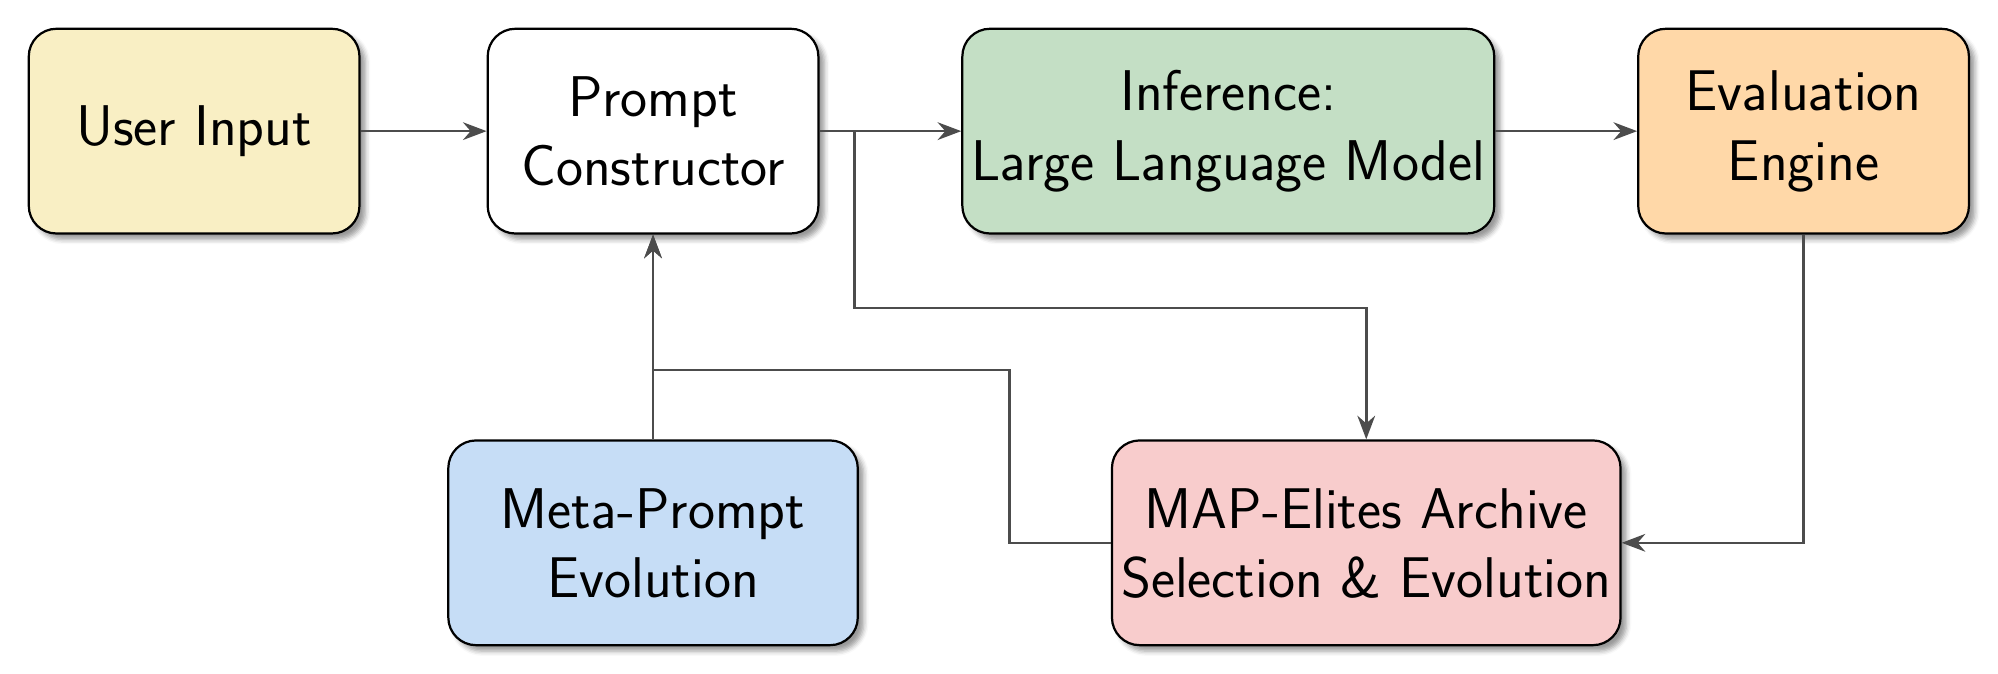
\begin{tikzpicture}[
			node distance=2.0cm and 2.0cm,
			every node/.style={font=\sffamily\huge}
			]
			% --- Top row ---
			\node[box, fill=pastelYellow] (input) {User Input};
			\node[box, fill=white] (prompt) [right=1.6cm of input] {Prompt\\Constructor};
			\node[box, fill=pastelGreen] (lm) [right=1.8cm of prompt] {Inference:\\ Large Language Model};
			\node[box, fill=pastelOrange] (eval) [right=1.8cm of lm] {Evaluation\\ Engine};
			
			% --- Bottom row (same level for RAG and Selection) ---
			% Place both with the same vertical offset so they align perfectly.
			\def\RowDrop{2.6cm}
			\node[box, fill=pastelBlue, minimum width=5.2cm] (rag)
			[below=\RowDrop of prompt] {Meta-Prompt\\Evolution};
			\node[box, fill=pastelRed] (select)
			 [right=3.2cm of rag]{MAP-Elites Archive\\ Selection \& Evolution};
			
			% --- Flows ---
			\draw[flow] (input) -- (prompt);
			\draw[flow] (prompt) -- (lm);
			\draw[flow] (lm) -- (eval);
			%\draw[flow] (select.west) -- (rag.east); % [yshift=-4pt]
			\draw[flow] (rag.north) -- (prompt.south);
			
			% 3) Selection -> LM: enter at the top-left corner (orthogonal)
			\draw[flow] (prompt.east) -| ($(lm)!0.65!(prompt) $) |- ($(rag)!0.57!(lm) $) -| (select.north);
			\draw[flow] (eval.south) |- (select.east);
			
			
			\draw[flow] (select.west) -|  ($(rag)!0.5!(select) $) |- ($(rag)!0.42!(prompt) $) -|  (prompt.south);
		\end{tikzpicture}%
	}%
}
    
\newcommand{\PipelineDiagramB}{%
	\resizebox{\linewidth}{!}{%
		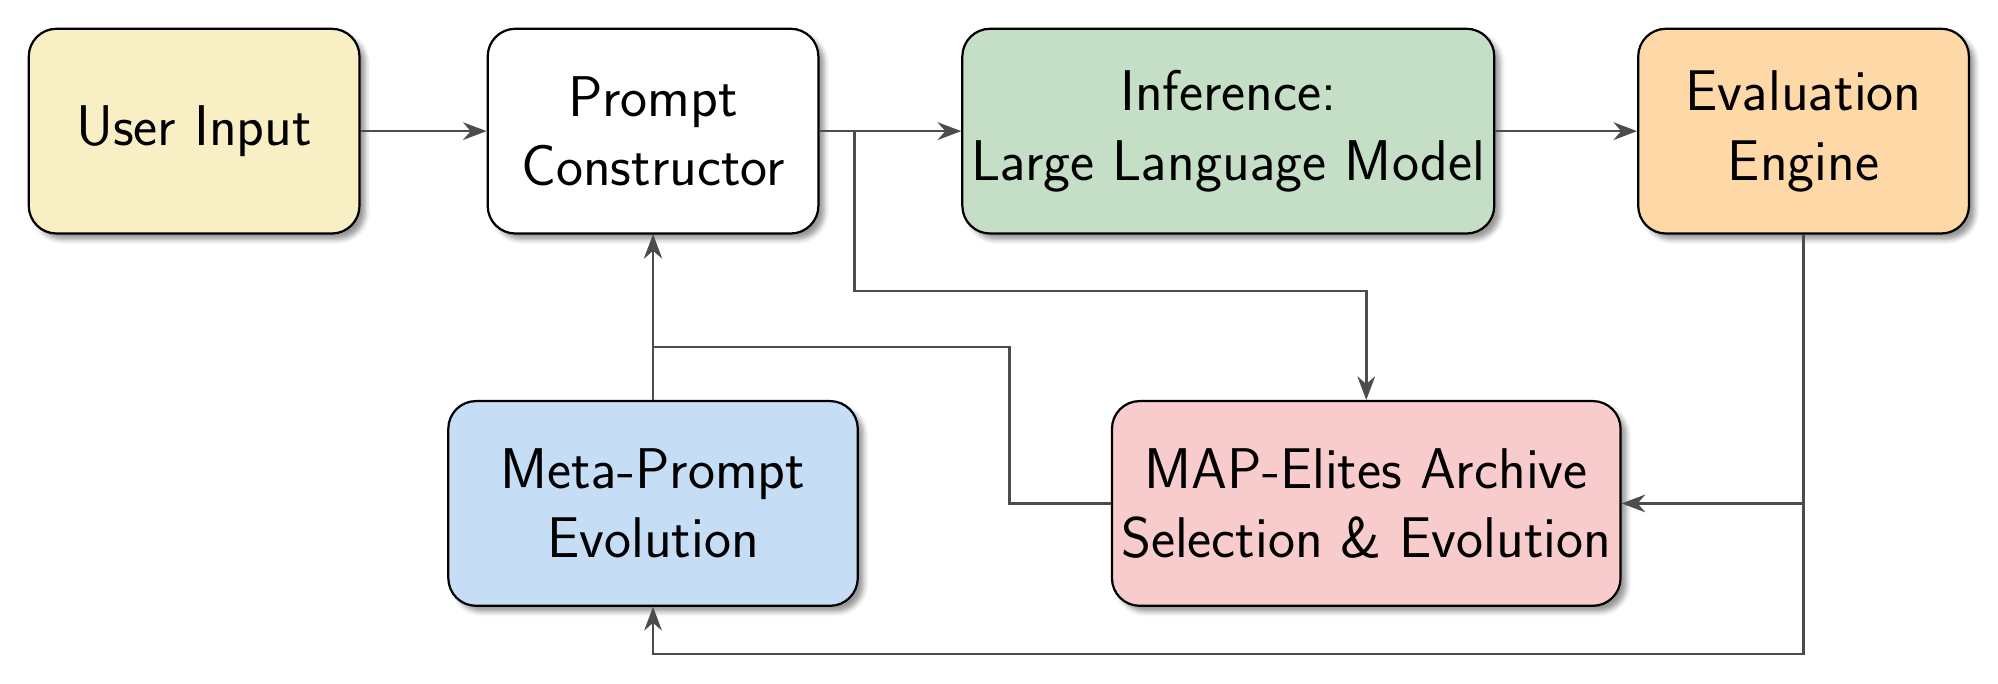
\begin{tikzpicture}[
			node distance=2.0cm and 2.0cm,
			every node/.style={font=\sffamily\huge}
			]
			% --- Top row ---
			\node[box, fill=pastelYellow] (input) {User Input};
			\node[box, fill=white] (prompt) [right=1.6cm of input] {Prompt\\Constructor};
			\node[box, fill=pastelGreen] (lm) [right=1.8cm of prompt] {Inference:\\ Large Language Model};
			\node[box, fill=pastelOrange] (eval) [right=1.8cm of lm] {Evaluation\\ Engine};
			
			% --- Bottom row (same level for RAG and Selection) ---
			% Place both with the same vertical offset so they align perfectly.
			\def\RowDrop{2.1cm}
			\node[box, fill=pastelBlue, minimum width=5.2cm] (rag)
			[below=\RowDrop of prompt] {Meta-Prompt\\Evolution};
			\node[box, fill=pastelRed] (select)
			 [right=3.2cm of rag]{MAP-Elites Archive\\ Selection \& Evolution};
			
			% --- Flows ---
			\draw[flow] (input) -- (prompt);
			\draw[flow] (prompt) -- (lm);
			\draw[flow] (lm) -- (eval);
			%\draw[flow] (select.west) -- (rag.east); % [yshift=-4pt]
			\draw[flow] (rag.north) -- (prompt.south);
			
			% 3) Selection -> LM: enter at the top-left corner (orthogonal)
			\draw[flow] (prompt.east) -| ($(lm)!0.65!(prompt) $) |- ($(rag)!0.57!(lm) $) -| (select.north);
			\draw[flow] (eval.south) |- (select.east);
			\draw[flow] (eval.south) |- ($(rag.south)-(0,6mm) $) -- (rag.south);
			
			
			\draw[flow] (select.west) -|  ($(rag)!0.5!(select) $) |- ($(rag)!0.42!(prompt) $) -|  (prompt.south);
		\end{tikzpicture}%
	}%
}

% --- colors ---
\definecolor{ragblue}{RGB}{198,221,246}
\definecolor{hardwareblue}{RGB}{176,196,222}
\definecolor{promptyellow}{RGB}{249,239,196}
\definecolor{infergreen}{RGB}{196,223,197}
\definecolor{evalorange}{RGB}{255,216,168}
\definecolor{dbred}{RGB}{248,204,204}
\definecolor{framegray}{RGB}{120,120,120}
\definecolor{textgray}{RGB}{60,60,60}

% --- macro ---
\newcommand{\OptimDiagram}{%
	\resizebox{0.95\linewidth}{!}{%
		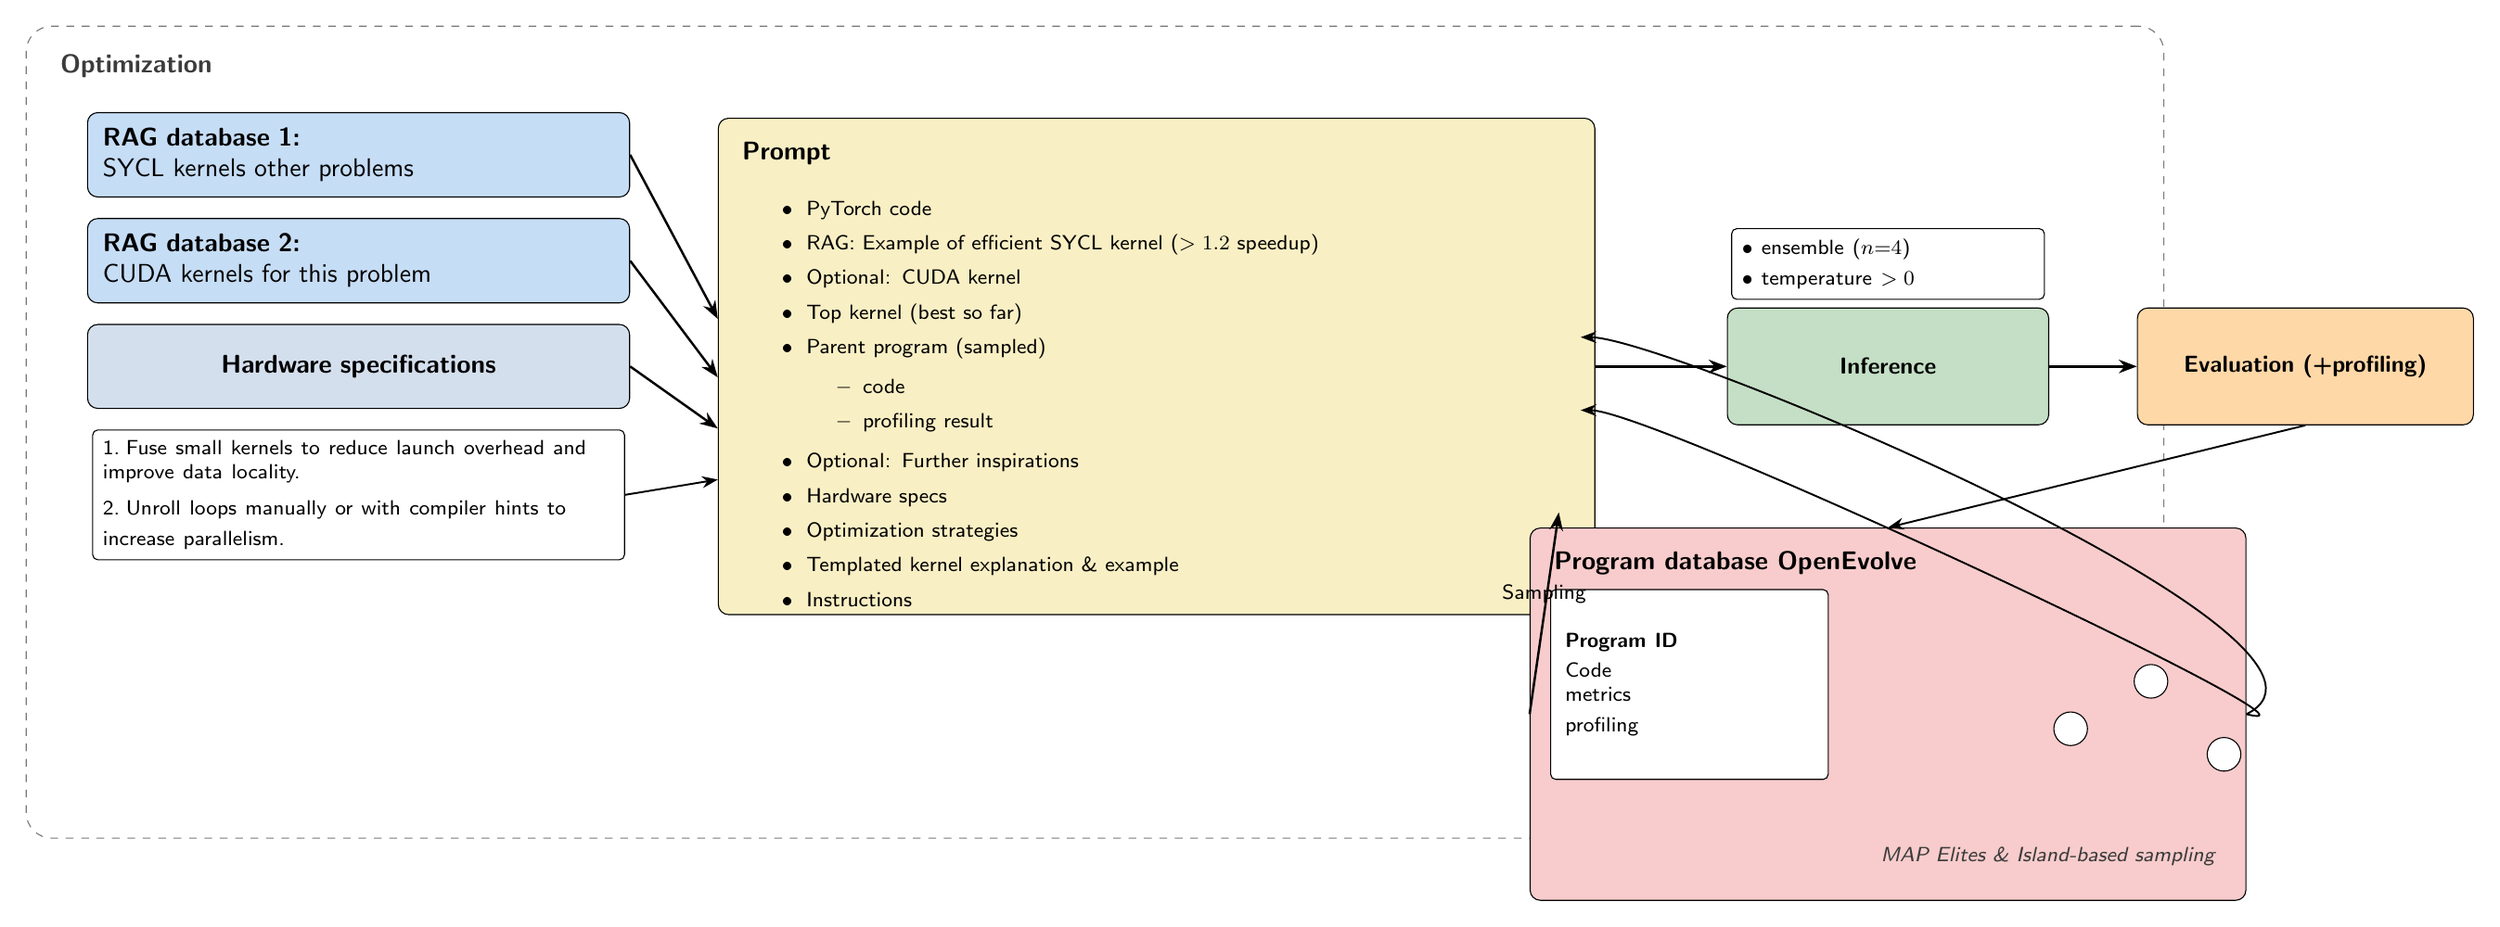
\begin{tikzpicture}[
			font=\sffamily,
			>=Stealth,
			line/.style={-Stealth, line width=0.9pt},
			thinarrow/.style={-Stealth, line width=0.7pt},
			note/.style={draw=black, fill=white, rounded corners=2pt, inner sep=4pt},
			box/.style={draw=black, rounded corners=4pt, inner sep=6pt},
			title/.style={font=\sffamily\bfseries},
			small/.style={font=\sffamily\footnotesize}
			]
			
			% --- outer dashed frame ---
			\node[draw=framegray, dashed, rounded corners=10pt,
			inner xsep=18pt, inner ysep=16pt,
			fit={(0,0) (28,10)}] (frame) {};
			\node[anchor=north west, title, text=textgray]
			at ($(frame.north west)+(10pt,-8pt)$) {Optimization};
			
			% --- left column ---
			\coordinate (L0) at (0.2,8.8);
			
			\node[box, fill=ragblue, minimum width=7.2cm, minimum height=1.15cm, anchor=west] (rag1) at (L0)
			[align=left,text width=7.0cm] {\textbf{RAG database 1:}\\ SYCL kernels other problems};
			
			\node[box, fill=ragblue, minimum width=7.2cm, minimum height=1.15cm, anchor=west, below=8pt of rag1.south] (rag2)
			[align=left,text width=7.0cm] {\textbf{RAG database 2:}\\ CUDA kernels for this problem};
			
			\node[box, fill=hardwareblue!55, minimum width=7.2cm, minimum height=1.15cm, anchor=west, below=8pt of rag2.south] (hw)
			[align=center,text width=7.0cm] {\textbf{Hardware specifications}};
			
			\node[note, minimum width=7.2cm, anchor=west, below=8pt of hw.south, align=left, text width=7.0cm] (hwnote) {%
				\footnotesize 1.\;Fuse small kernels to reduce launch overhead and improve data locality.\\[2pt]
				2.\;Unroll loops manually or with compiler hints to increase parallelism.
			};
			
			% --- prompt box ---
			\node[box, fill=promptyellow, minimum width=12cm, minimum height=6.8cm,
			anchor=west, right=1.2cm of hw.east] (prompt) {};
			
			\node[anchor=north west, title] at ($(prompt.north west)+(6pt,-6pt)$) {Prompt};
			
			\node[anchor=north west, small, align=left, text width=11.3cm]
			at ($(prompt.north west)+(6pt,-22pt)$) (promptlist) {%
				\begin{itemize}\itemsep=2pt
					\item PyTorch code
					\item RAG: Example of efficient SYCL kernel ($>1.2$ speedup)
					\item Optional: CUDA kernel
					\item Top kernel (best so far)
					\item Parent program (sampled)
					\begin{itemize}\itemsep=2pt
						\item code
						\item profiling result
					\end{itemize}
					\item Optional: Further inspirations
					\item Hardware specs
					\item Optimization strategies
					\item Templated kernel explanation \& example
					\item Instructions
				\end{itemize}
			};
			
			% tap points along prompt's west edge
			\coordinate (p_w1) at ($(prompt.west)+(0,  0.65)$);
			\coordinate (p_w2) at ($(prompt.west)+(0, -0.15)$);
			\coordinate (p_w3) at ($(prompt.west)+(0, -0.85)$);
			\coordinate (p_w4) at ($(prompt.west)+(0, -1.55)$);
			
			% arrows from left into prompt
			\draw[line] (rag1.east) -- (p_w1);
			\draw[line] (rag2.east) -- (p_w2);
			\draw[line] (hw.east)   -- (p_w3);
			\draw[thinarrow] (hwnote.east) -- (p_w4);
			
			% --- inference ---
			\node[box, fill=infergreen, minimum width=4.4cm, minimum height=1.6cm,
			anchor=west, right=1.8cm of prompt.east] (infer)
			{\small\textbf{Inference}};
			
			\node[note, anchor=south, above=3pt of infer.north, align=left, text width=4.0cm] (infernote) {\footnotesize
				$\bullet$ ensemble ($n{=}4$)\\
				$\bullet$ temperature $> 0$
			};
			
			\draw[line] (prompt.east) -- (infer.west);
			
			% --- evaluation ---
			\node[box, fill=evalorange, minimum width=4.6cm, minimum height=1.6cm,
			anchor=west, right=1.2cm of infer.east] (eval)
			{\small\textbf{Evaluation (+profiling)}};
			
			\draw[line] (infer.east) -- (eval.west);
			
			% --- program database ---
			\node[box, fill=dbred, minimum width=9.8cm, minimum height=5.1cm,
			anchor=north, below=1.4cm of infer.south] (db) {};
			
			\node[anchor=north west, title] at ($(db.north west)+(6pt,-6pt)$)
			{Program database \textit{OpenEvolve}};
			
			\node[draw=black, fill=white, rounded corners=2pt,
			minimum width=3.8cm, minimum height=2.6cm,
			anchor=north west, align=left, text width=3.4cm]
			at ($(db.north west)+(8pt,-24pt)$) (dbinfo) {\footnotesize
				\textbf{Program ID}\\[2pt]
				Code\\
				metrics\\
				profiling
			};
			
			% white circles (islands)
			\draw[fill=white, draw=black] ($(db.center)+(2.5cm,-0.2cm)$) circle [radius=0.23cm];
			\draw[fill=white, draw=black] ($(db.center)+(3.6cm, 0.45cm)$) circle [radius=0.23cm];
			\draw[fill=white, draw=black] ($(db.center)+(4.6cm,-0.55cm)$) circle [radius=0.23cm];
			
			\node[small, anchor=south east, text=textgray]
			at ($(db.south east)+(-8pt,10pt)$)
			{\textit{MAP Elites \& Island-based sampling}};
			
			\draw[thinarrow] (eval.south) -- ($(db.north)+(0.0,0.0)$);
			\draw[line] (db.west) -- node[above, small] {Sampling} ($(prompt.east)+(-0.5, -2.0)$);
			
			% optional leftward sampling hints
			\draw[thinarrow] (db.east) .. controls ($(db.east)+(2.0,1.0)$) and ($(prompt.east)+(1.0,0.4)$) .. ($(prompt.east)+(-0.2,0.4)$);
			\draw[thinarrow] (db.east) .. controls ($(db.east)+(1.6,-0.4)$) and ($(prompt.east)+(0.8,-0.6)$) .. ($(prompt.east)+(-0.2,-0.6)$);
			
		\end{tikzpicture}%
	}%
}

% blues colormap definition (sample points from the colormap)
\definecolor{blues0}{RGB}{240,252,255}
\definecolor{blues1}{RGB}{205,244,250}
\definecolor{blues2}{RGB}{170,235,244}
\definecolor{blues3}{RGB}{135,225,235}
\definecolor{blues4}{RGB}{100,215,228}
\definecolor{blues5}{RGB}{65,205,220}
\definecolor{blues6}{RGB}{45,185,200}
\definecolor{blues7}{RGB}{35,165,182}
\definecolor{blues8}{RGB}{30,145,165}
\definecolor{blues9}{RGB}{25,125,148}

% Default z-spacing for flat tiles
\newcommand{\flattilezspacing}{0.5}

\tikzset{
	get flat projections/.style={insert path={%
			let \p1=(1,0,0),\p2=(0,1,0)  in 
			[/utils/exec={\pgfmathtruncatemacro{\xproj}{sign(\x1)}\xdef\xproj{\xproj}
				\pgfmathtruncatemacro{\yproj}{sign(\x2)}\xdef\yproj{\yproj}
				\pgfmathtruncatemacro{\zproj}{sign(cos(\tdplotmaintheta))}\xdef\zproj{\zproj}}]}},
	pics/flat tile/.style={code={
			\path[get flat projections];
			% Generate random blues color for this tile
			\pgfmathtruncatemacro{\tilecoloridx}{random(0,9)}
			% Draw thin tile (just the top face as a filled rectangle)
			\fill[3d cube/every face,fill=blues\tilecoloridx] (0,0,0) -- (1,0,0) -- (1,1,0) -- (0,1,0) -- cycle; 
	}},
	3d cube/.cd,
	xy face/.style={fill=ragblue!100},
	xz face/.style={fill=ragblue!180},
	yz face/.style={fill=ragblue!255},
	num cubes x/.estore in=\NumCubesX,
	num cubes y/.estore in=\NumCubesY,
	num cubes z/.estore in=\NumCubesZ,
	num cubes x=1,num cubes y/.initial=1,num cubes z/.initial=1,
	cube scale/.initial=0.9,
	z spacing/.initial=1.75,  % Controls spacing between z-layers
	every face/.style={draw},
	/tikz/pics/.cd,
	flat cube array/.style={code={%
			\tikzset{3d cube/.cd,#1}%
			\pgfmathsetmacro{\flattilezspacingval}{\pgfkeysvalueof{/tikz/3d cube/z spacing}}%
			\xdef\flattilezspacing{\flattilezspacingval}%
			\path[get flat projections];
			\ifnum\yproj=1
			\def\LstX{1,...,\NumCubesX}
			\else 
			\ifnum\NumCubesX>1
			\pgfmathtruncatemacro{\NextToLast}{\NumCubesX-1}
			\def\LstX{\NumCubesX,\NextToLast,...,1}
			\else
			\def\LstX{1}   
			\fi 
			\fi
			\ifnum\xproj=-1
			\def\LstY{1,...,\NumCubesY}
			\else 
			\ifnum\NumCubesY>1
			\pgfmathtruncatemacro{\NextToLast}{\NumCubesY-1}
			\def\LstY{\NumCubesY,\NextToLast,...,1}
			\else
			\def\LstY{1}   
			\fi 
			\fi
			\ifnum\zproj=1
			\def\LstZ{1,...,\NumCubesZ}
			\else 
			\ifnum\NumCubesZ>1
			\pgfmathtruncatemacro{\NextToLast}{\NumCubesZ-1}
			\def\LstZ{\NumCubesZ,\NextToLast,...,1}
			\else
			\def\LstZ{1}   
			\fi 
			\fi
			\foreach \X in \LstX
			{\foreach \Y in \LstY
				{\foreach \Z in \LstZ
					{\path (\X-\NumCubesX/2-1,\Y-\NumCubesY/2-1,{(\Z-\NumCubesZ/2-1)*\flattilezspacing})
						pic[scale=\pgfkeysvalueof{/tikz/3d cube/cube scale}]{flat tile};}}
			}
	}},
}

% ============================================================================
% QD-GRADIENT MAP-ELITES VISUALIZATION SYSTEM
% ============================================================================
%
% Production-ready TikZ visualization for Quality-Diversity evolutionary
% algorithms with gradient-based enhancements.
%
% Based on the 4D behavioral space from qd_gradient.py:
%   - memory_opt (0-3): Memory hierarchy exploitation level
%   - compute_opt (0-3): Algorithmic efficiency level  
%   - parallelism_opt (0-3): Parallelism granularity level
%   - esimd_opt (0-3): ESIMD vectorization level
%
% Visualization modes:
%   1. 3D Grid: Standard MAP-Elites archive visualization
%   2. 4D Sliced: Multiple 2D slices showing 4th dimension
%   3. Transition Flow: Parent→child evolutionary transitions
%   4. Gradient Field: Estimated gradient directions
%   5. Coverage Heatmap: Archive coverage analysis
%
% ============================================================================

% ----------------------------------------------------------------------------
% Additional colors for QD visualization
% ----------------------------------------------------------------------------
\definecolor{qdEmpty}{RGB}{245,245,245}           % Empty cell background
\definecolor{qdElite}{RGB}{255,223,0}             % Elite marker (gold)
\definecolor{qdParent}{RGB}{65,105,225}           % Parent selection (royal blue)
\definecolor{qdChild}{RGB}{50,205,50}             % Child placement (lime green)
\definecolor{qdImprovement}{RGB}{34,139,34}       % Improvement transition
\definecolor{qdRegression}{RGB}{220,20,60}        % Regression transition
\definecolor{qdNeutral}{RGB}{169,169,169}         % Neutral transition
\definecolor{qdExploration}{RGB}{255,140,0}       % Exploration gradient
\definecolor{qdGradientPos}{RGB}{0,128,0}         % Positive gradient direction
\definecolor{qdGradientNeg}{RGB}{178,34,34}       % Negative gradient direction

% ----------------------------------------------------------------------------
% QD Cell Styles
% ----------------------------------------------------------------------------
\tikzset{
	% Base cell style
	qd cell/.style={
		draw=black!40,
		line width=0.3pt,
		minimum size=0.8cm,
	},
	% Empty/unoccupied niche
	qd empty cell/.style={
		qd cell,
		fill=qdEmpty,
		pattern=north east lines,
		pattern color=black!10,
	},
	% Occupied cell with fitness coloring (use with fill=bluesN)
	qd occupied cell/.style={
		qd cell,
		line width=0.5pt,
	},
	% Elite cell marker
	qd elite cell/.style={
		qd occupied cell,
		line width=1.2pt,
		draw=qdElite,
	},
	% Currently selected parent
	qd parent cell/.style={
		qd occupied cell,
		line width=1.5pt,
		draw=qdParent,
	},
	% Newly placed child
	qd child cell/.style={
		qd occupied cell,
		line width=1.5pt,
		draw=qdChild,
	},
	% Transition arrow styles
	qd transition/.style={
		-{Stealth[length=2mm,width=1.5mm]},
		line width=0.8pt,
		opacity=0.7,
	},
	qd improvement/.style={
		qd transition,
		draw=qdImprovement,
		line width=1.2pt,
	},
	qd regression/.style={
		qd transition,
		draw=qdRegression,
		dashed,
	},
	qd neutral/.style={
		qd transition,
		draw=qdNeutral,
		dotted,
	},
	% Gradient arrow style
	qd gradient arrow/.style={
		-{Stealth[length=2.5mm,width=2mm]},
		line width=1pt,
		draw=qdExploration,
	},
}

% ----------------------------------------------------------------------------
% HELPER: blues color interpolation
% ----------------------------------------------------------------------------
% #1: value between 0 and 1
% Result: sets \bluescolor to the interpolated color
\newcommand{\getbluesColor}[1]{%
	\pgfmathsetmacro{\colorpos}{#1*9}%
	\pgfmathtruncatemacro{\loweridx}{min(floor(\colorpos),8)}%
	\pgfmathtruncatemacro{\upperidx}{\loweridx+1}%
	\pgfmathsetmacro{\blend}{100-(\colorpos-\loweridx)*100}%
	\colorlet{bluescolor}{blues\loweridx!\blend!blues\upperidx}%
}

% ----------------------------------------------------------------------------
% HELPER: Draw fitness colorbar
% ----------------------------------------------------------------------------
% #1: x position, #2: y position, #3: height, #4: title
\newcommand{\QDColorbar}[4]{%
	\begin{scope}[xshift=#1, yshift=#2]
		% Smooth continuous gradient
		\pgfmathsetmacro{\stepheight}{#3/20}%
		\foreach \i in {0,...,19} {
			\pgfmathsetmacro{\fraction}{\i/19}%
			\getbluesColor{\fraction}%
			\fill[bluescolor] (0, \i*\stepheight) rectangle (0.3, \i*\stepheight+\stepheight);
		}
		\draw[black!50, line width=0.5pt] (0, 0) rectangle (0.3, #3);
		% Labels
		\node[font=\sffamily\tiny, anchor=east] at (-0.08, 0) {0.0};
		\node[font=\sffamily\tiny, anchor=east] at (-0.08, #3*0.25) {0.25};
		\node[font=\sffamily\tiny, anchor=east] at (-0.08, #3*0.5) {0.5};
		\node[font=\sffamily\tiny, anchor=east] at (-0.08, #3*0.75) {0.75};
		\node[font=\sffamily\tiny, anchor=east] at (-0.08, #3) {1.0};
		% Title
		\node[font=\sffamily\footnotesize, anchor=south, rotate=90] at (0.7, #3*0.5) {#4};
	\end{scope}%
}

% ============================================================================
% OPTION A: MAPElitesGridCorrected - Full pipeline with accurate flow
% ============================================================================
% A corrected version that shows: Prompt Constructor, Compilation, Execution,
% Behavioral Classification, and proper feedback integration.
% Arguments: #1-#3: axis labels, #4-#6: grid dimensions, #7: random seed
\newcommand{\MAPElitesGridCorrected}[7]{%
    \begin{tikzpicture}[font=\sffamily\scriptsize, remember picture]
        % Pre-compute loop bounds
        \pgfmathtruncatemacro{\cellsX}{#4}%
        \pgfmathtruncatemacro{\cellsY}{#5}%
        \pgfmathtruncatemacro{\cellsZ}{#6}%
        \pgfmathtruncatemacro{\loopXmax}{\cellsX-1}%
        \pgfmathtruncatemacro{\loopYmax}{\cellsY-1}%
        \pgfmathtruncatemacro{\loopZmax}{\cellsZ-1}%
        
        % =========================================================================
        % MAIN EVOLUTIONARY LOOP (top section - horizontal flow)
        % =========================================================================
        % Row 1: Selection -> Prompt Constructor -> LLM
        \node[draw, rounded corners, fill=pastelRed, minimum height=0.7cm, 
              minimum width=1.4cm, align=center] (selection) at (0, 3.5) {Elite\\Selection};
        
        \node[draw, rounded corners, fill=white, minimum height=0.7cm, 
              minimum width=1.6cm, align=center, right=0.5cm of selection] (prompt) {Prompt\\Constructor};
        
        \node[draw, rounded corners, fill=pastelGreen, minimum height=0.7cm, 
              minimum width=1.4cm, align=center, right=0.5cm of prompt] (llm) {Inference:\\Large Language Model};
        
        % Row 2: Compilation -> Execution -> Classification -> Archive Update
        \node[draw, rounded corners, fill=pastelOrange, minimum height=0.7cm, 
              minimum width=1.4cm, align=center, right=0.5cm of llm] (compile) {Compile};
        
        \node[draw, rounded corners, fill=pastelOrange, minimum height=0.7cm, 
              minimum width=1.4cm, align=center, below=0.5cm of compile] (execute) {Execute\\ \& \\Profile};
        
        \node[draw, rounded corners, fill=pastelRed, minimum height=0.7cm, 
              minimum width=1.6cm, align=center, below=0.5cm of execute] (classify) {Behavioral\\Classifier};
        
        \node[draw, rounded corners, fill=pastelRed, minimum height=0.7cm, 
              minimum width=1.4cm, align=center, below=0.5cm of classify] (update) {Archive\\Update};
        
        % Main flow arrows
        \draw[-Stealth, thick] (selection) -- (prompt);
        \draw[-Stealth, thick] (prompt) -- (llm);
        \draw[-Stealth, thick] (llm) -- (compile);
        \draw[-Stealth, thick] (compile) -- (execute);
        \draw[-Stealth, thick] (execute) -- (classify);
        \draw[-Stealth, thick] (classify) -- (update);
        
        % Compilation failure feedback loop (back to LLM)
        \draw[-Stealth, thick, dashed, red!60] (compile.north) -- ++(0, 0.4) 
            -| node[pos=0.25, above, font=\tiny\itshape, red] {Compile error} (llm.north);
        
        % =========================================================================
        % EXTERNAL INPUTS (feeding into Prompt Constructor)
        % =========================================================================
        \node[draw, rounded corners, fill=pastelBlue, minimum height=0.5cm,
              align=center] (meta) at ($(prompt.north)+(0.0, 0.85)$) {Meta-Prompt\\Evolution};
    
        \draw[-Stealth, thick] (meta.south) -- ($(prompt.north)+(0.0, 0)$);

        \draw[-Stealth, thick] (execute.east) -- ++(0.5, 0.0) 
            |- (meta.east);
        
        % =========================================================================
        % PROFILER FEEDBACK (from Execute back to Prompt)
        % =========================================================================
        
        % \draw[-Stealth, thick] (execute.west) -| ($(prompt.south)+(0, -0.3)$) 
        %     -- ($(prompt.south)+(0, 0)$)
        %     node[pos=-1.5, right, font=\tiny\itshape] {Profiler feedback};
        
        % =========================================================================
        % TRANSITION TRACKER (from Update)
        % =========================================================================
        \node[draw, rounded corners, fill=pastelPurple, minimum height=0.6cm,
              align=center, right=2.25cm of update] (tracker) {Transition\\Tracker};
        
        \draw[-Stealth, thick] (update) -- (tracker) node[midway, above, font=\tiny\itshape] {record};
        
        % =========================================================================
        % GRADIENT ESTIMATOR (below tracker)
        % =========================================================================
        \node[draw, rounded corners, fill=pastelPurple, minimum height=0.6cm,
              align=center, above=0.6cm of tracker] (estimator) {Gradient\\Estimator};
        
        % Three gradient components
        \node[draw, rounded corners, fill=pastelPurple!30, font=\tiny,
              above left=0.4cm and 0.1cm of estimator] (nablaF) {$\nabla_F$};
        \node[draw, rounded corners, fill=pastelPurple!30, font=\tiny,
              above=0.4cm of estimator] (nablaR) {$\nabla_R$};
        \node[draw, rounded corners, fill=pastelPurple!30, font=\tiny,
              above right=0.4cm and 0.1cm of estimator] (nablaE) {$\nabla_E$};
        
        % Combined gradient output
        \node[draw, rounded corners, fill=pastelPurple!20, font=\tiny,
              above=0.4cm of nablaR, minimum width=2.4cm, align=center] (combined) {
            $\nabla = \alpha\nabla_F + \beta\nabla_R + \gamma\nabla_E$
        };
        
        \draw[-Stealth, thick] (tracker) -- (estimator);
        \draw[-Stealth, thick] (estimator) -- (nablaF);
        \draw[-Stealth, thick] (estimator) -- (nablaR);
        \draw[-Stealth, thick] (estimator) -- (nablaE);
        \draw[-Stealth, thick] (nablaF) -- (combined);
        \draw[-Stealth, thick] (nablaR) -- (combined);
        \draw[-Stealth, thick] (nablaE) -- (combined);
        
        % Gradient feedback to Selection (sampling weights)
        \draw[-Stealth, thick] (combined.north) -- ++(0, 2.4) 
            -|  (selection.north)
            node[pos=0.7, left, align=center, font=\tiny\itshape] {Sampling\\weights};
            
        \QDColorbar{3.8cm}{-1.5cm}{3.0}{Fitness}
        % =========================================================================
        % 3D BEHAVIORAL ARCHIVE GRID
        % =========================================================================
        \tdplotsetmaincoords{80}{40}
        \begin{scope}[tdplot_main_coords]
            \pgfmathsetseed{#7}
            \pgfmathsetmacro{\cubescale}{0.9}
            \pgfmathsetmacro{\zspacing}{1.15}
            \pgfmathsetmacro{\numX}{\cellsX}
            \pgfmathsetmacro{\numY}{\cellsY}
            \pgfmathsetmacro{\numZ}{\cellsZ}

            
            
            % Draw the behavioral archive grid
            \pic{qd flat cube array={num cubes x=\cellsX, num cubes y=\cellsY, 
                num cubes z=\cellsZ, z spacing=\zspacing, cube scale=\cubescale}};
            
            % Selected elite cells (highlighted)
            \coordinate (elite1) at (-1.6, -1.5, 1*\zspacing);
            \coordinate (elite2) at (-1.6, -1.5, -2*\zspacing);
            \coordinate (nichespot) at (1.75, 0.2, -1*\zspacing);
            
            % Axis bounds
            \pgfmathsetmacro{\xmin}{1-\numX/2-1}
            \pgfmathsetmacro{\xmax}{\numX-\numX/2}
            \pgfmathsetmacro{\ymin}{1-\numY/2-1}
            \pgfmathsetmacro{\ymax}{\numY-\numY/2}
            \pgfmathsetmacro{\zmin}{(1-\numZ/2-1)*\zspacing}
            \pgfmathsetmacro{\zmax}{(\numZ-\numZ/2)*\zspacing}
            
            % Axes
            \draw[-Stealth, thick, black!70] (\xmin-0.3, \ymin-0.3, \zmin) 
                -- (\xmax+0.5, \ymin-0.3, \zmin) 
                node[pos=1.05, anchor=west, font=\sffamily\footnotesize] {#1};
            \draw[-Stealth, thick, black!70] (\xmin-0.3, \ymin-0.3, \zmin) 
                -- (\xmin-0.3, \ymax+0.5, \zmin) 
                node[pos=0.6, anchor=south, font=\sffamily\footnotesize] {#2};
            \draw[-Stealth, thick, black!70] (\xmin-0.3, \ymin-0.3, \zmin) 
                -- (\xmin-0.3, \ymin-0.3, \zmax-1.25) 
                node[pos=1.05, anchor=south, font=\sffamily\footnotesize] {#3};
            
            % Tick marks
            \foreach \i in {0,...,\loopXmax} {
                \pgfmathsetmacro{\xpos}{\i+1-\numX/2-1+0.5}
                \node[font=\sffamily\tiny, anchor=north] at (\xpos, \ymin-0.4, \zmin) {\i};
            }
            \foreach \i in {0,...,\loopYmax} {
                \pgfmathsetmacro{\ypos}{\i+1-\numY/2-1+0.5}
                \node[font=\sffamily\tiny, anchor=east] at (\xmin-0.4, \ypos, \zmin+0.1) {\i};
            }
            \foreach \i in {0,...,\loopZmax} {
                \pgfmathsetmacro{\zpos}{(\i+1-\numZ/2-1)*\zspacing}
                \node[font=\sffamily\tiny, anchor=east] at (\xmin-0.4, \ymin-0.3, \zpos) {\i};
            }
        \end{scope}
        
        % =========================================================================
        % GRID CONNECTIONS
        % =========================================================================
        % Elites -> Selection (sampling from archive)
        \draw[-Stealth, thick] (elite1) 
            to[out=90, in=-120, looseness=0.8] (selection.south);
        \draw[-Stealth, thick] (elite2) 
            to[out=90, in=-60, looseness=0.6] (selection.south);
        
        % Update -> Grid (archive insertion)
        \draw[-Stealth, thick] (update.south) 
            to[out=-90, in=90] (nichespot);
        
        % =========================================================================
        % LEGEND (bottom right)
        % =========================================================================
        % \node[font=\sffamily\scriptsize, align=left, anchor=north west] at (8.5, -1.9) {
        %     \textcolor{black}{---} Main flow\\
        %     \textcolor{red}{- -} Error feedback\\
        %     \textcolor{orange}{---} Profiler feedback\\
        %     \textcolor{purple}{---} Gradient guidance
        % };
        
    \end{tikzpicture}%
}

% ============================================================================
% OPTION B: GradientInformedEvolution - Focused on the gradient mechanism
% ============================================================================
% A clean, focused figure showing only the gradient-informed evolution mechanism:
% Transition tracking, gradient estimation, and how it influences selection.
% Arguments: #1: grid size for 2D slice, #2: random seed
\newcommand{\GradientInformedEvolution}[2]{%
    \begin{tikzpicture}[font=\sffamily\small]
        \pgfmathtruncatemacro{\gridSize}{#1}%
        \pgfmathsetseed{#2}%
        
        % =========================================================================
        % LEFT: 2D Behavioral Archive Slice with Transitions
        % =========================================================================
        \begin{scope}[shift={(0, 0)}]
            \node[font=\sffamily\bfseries\footnotesize, anchor=south] at (2, 3.0) 
                {Behavioral Archive (2D slice)};
            
            % Draw grid
            \foreach \x in {0,...,3} {
                \foreach \y in {0,...,3} {
                    % Randomly determine if cell is occupied and its fitness
                    \pgfmathparse{random()}%
                    \pgfmathsetmacro{\isOccupied}{\pgfmathresult}%
                    \pgfmathparse{random()}%
                    \pgfmathsetmacro{\fitness}{\pgfmathresult}%
                    \ifnum\pdfstrcmp{\isOccupied}{0.4}>0
                        \getbluesColor{\fitness}%
                        \fill[bluescolor, draw=black!40, line width=0.5pt] 
                            (\x, \y) rectangle (\x+1, \y+1);
                        % Fitness value
                        \pgfmathtruncatemacro{\fitPercent}{\fitness*100}%
                    \else
                        \fill[white, draw=black!20, line width=0.5pt] 
                            (\x, \y) rectangle (\x+1, \y+1);
                    \fi
                }
            }
            
            % Highlight specific cells for the example
            % Parent cell (yellow border)
            \draw[yellow!80!orange, line width=2pt] (1, 2) rectangle (2, 3);
            \node[font=\tiny, yellow!80!orange] at (1.5, 2.5) {\textbf{P}};
            
            % Child cell (green border) - successful transition
            \draw[green!70!black, line width=2pt] (2, 3) rectangle (3, 4);
            \node[font=\tiny, green!70!black] at (2.5, 3.5) {\textbf{C}};
            
            % Transition arrow
            \draw[-Stealth, thick, green!60!black, line width=1.5pt] 
                (1.7, 2.7) -- (2.3, 3.3)
                node[midway, above left, font=\tiny] {$+\Delta f$};
            
            % Failed transition (dashed, to empty cell)
            \draw[-Stealth, dashed, red!60, line width=1pt] 
                (1.5, 2.2) -- (0.5, 1.5);
            
            % Axis labels
            \draw[-Stealth, thick, black!70] (-0.3, -0.3) -- (4.5, -0.3) 
                node[pos=1.0, anchor=west, font=\footnotesize] {$d_{\text{mem}}$};
            \draw[-Stealth, thick, black!70] (-0.3, -0.3) -- (-0.3, 4.5) 
                node[pos=1.0, anchor=south, font=\footnotesize] {$d_{\text{algo}}$};
            
            % Colorbar
            \QDColorbar{4.8cm}{0cm}{4.0}{Fitness}
        \end{scope}
        
        % =========================================================================
        % CENTER: Transition Tracker
        % =========================================================================
        \begin{scope}[shift={(7.5, 0)}]
            \node[draw, rounded corners, fill=pastelRed!70, minimum height=0.8cm,
                  minimum width=3cm, align=center, font=\bfseries\footnotesize] 
                  (tracker) at (0, 4.2) {Transition Tracker};
            
            % Circular buffer visualization
            \node[draw, rounded corners, fill=pastelYellow!50, 
                  minimum width=2.8cm, minimum height=2.5cm, align=left, font=\tiny,
                  below=0.3cm of tracker] (buffer) {
                \texttt{buffer[0]:}\\
                \quad $(1,2,0)\to(2,3,0)$\\
                \quad $\Delta f = +0.12$\\
                \quad outcome: improve\\[3pt]
                \texttt{buffer[1]:}\\
                \quad $(1,2,0)\to(0,1,0)$\\
                \quad $\Delta f = -0.05$\\
                \quad outcome: regress\\[3pt]
                \texttt{...}
            };
            
            % Direction statistics
            \node[draw, rounded corners, fill=pastelYellow!30,
                  minimum width=2.8cm, align=left, font=\tiny,
                  below=0.3cm of buffer] (stats) {
                \textbf{Cell (1,2,0) stats:}\\
                $\vec{d}=(+1,+1,0)$: 3/5 success\\
                $\vec{d}=(-1,-1,0)$: 1/4 success\\
                $\vec{d}=(+1,0,0)$: 2/3 success
            };
            
            \draw[-Stealth, thick] (tracker) -- (buffer);
            \draw[-Stealth, thick] (buffer) -- (stats);
        \end{scope}
        
        % =========================================================================
        % RIGHT: Gradient Estimator
        % =========================================================================
        \begin{scope}[shift={(12.5, 0)}]
            \node[draw, rounded corners, fill=pastelPurple, minimum height=0.8cm,
                  minimum width=3cm, align=center, font=\bfseries\footnotesize] 
                  (estimator) at (0, 4.2) {Gradient Estimator};
            
            % Three gradient components with formulas
            \node[draw, rounded corners, fill=pastelPurple!40, 
                  minimum width=2.8cm, align=center, font=\tiny,
                  below=0.4cm of estimator] (fitgrad) {
                \textbf{Fitness Gradient} $\nabla_F$\\[2pt]
                $\displaystyle\sum_{\vec{d}} p(\vec{d}) \cdot \Delta f(\vec{d}) \cdot \vec{d}$
            };
            
            \node[draw, rounded corners, fill=pastelPurple!40,
                  minimum width=2.8cm, align=center, font=\tiny,
                  below=0.25cm of fitgrad] (impgrad) {
                \textbf{Improvement Rate} $\nabla_R$\\[2pt]
                $\displaystyle\sum_{\vec{d}} \frac{\text{success}(\vec{d})}{\text{total}(\vec{d})} \cdot \vec{d}$
            };
            
            \node[draw, rounded corners, fill=pastelPurple!40,
                  minimum width=2.8cm, align=center, font=\tiny,
                  below=0.25cm of impgrad] (expgrad) {
                \textbf{Exploration} $\nabla_E$\\[2pt]
                $\displaystyle\sum_{\vec{d}} (1 - \text{coverage}(\vec{d})) \cdot \vec{d}$
            };
            
            % Combined gradient
            \node[draw, rounded corners, fill=pastelPurple!20,
                  minimum width=2.8cm, align=center, font=\small,
                  below=0.35cm of expgrad] (combined) {
                $\nabla = \alpha\nabla_F + \beta\nabla_R + \gamma\nabla_E$
            };
            
            \draw[-Stealth, thick] (estimator) -- (fitgrad);
            \draw[-Stealth, thick] (fitgrad) -- (impgrad);
            \draw[-Stealth, thick] (impgrad) -- (expgrad);
            \draw[-Stealth, thick] (expgrad) -- (combined);
            
            % Default weights annotation
            \node[font=\tiny\itshape, anchor=west, text=black!60] 
                at ($(combined.east)+(0.1, 0)$) {$\alpha{=}0.4, \beta{=}0.4, \gamma{=}0.2$};
        \end{scope}
        
        % =========================================================================
        % ARROWS CONNECTING SECTIONS
        % =========================================================================
        % Archive -> Tracker (record transition)
        \draw[-Stealth, thick, black!70] (5.8, 3.5) -- (5.8, 4.2) -| (7.5-1.5, 4.2)
            node[pos=0.3, above, font=\tiny\itshape] {record transitions};
        
        % Stats -> Estimator
        \draw[-Stealth, thick, black!70] (7.5+1.4, 0.5) -- (12.5-1.4, 0.5) |- (12.5-1.4, 2.8)
            node[pos=0.3, below, font=\tiny\itshape] {direction stats};
        
        % Combined -> Selection guidance (back to archive)
        \draw[-Stealth, thick, orange!70, line width=1.2pt] 
            (combined.south) -- ++(0, -0.5) -| (-0.5, -0.8) -- (-0.5, 2.5) 
            node[pos=0.7, left, font=\tiny\itshape, text=orange!80] {sampling bias};
        
        % =========================================================================
        % OUTPUT BOX: What gradient informs
        % =========================================================================
        \node[draw, rounded corners, fill=pastelGreen!50, 
              minimum width=4cm, minimum height=1.2cm, align=left, font=\tiny,
              anchor=north west] at (7.5-1.5, -1.0) {
            \textbf{Gradient-Informed Decisions:}\\
            $\bullet$ Elite selection probability $\propto e^{\|\nabla\|}$\\
            $\bullet$ Mutation direction hints in prompt\\
            $\bullet$ Exploration vs exploitation balance
        };
        
    \end{tikzpicture}%
}

% ============================================================================
% CONVENIENCE WRAPPERS
% ============================================================================
\newcommand{\MAPElitesGridCorrectedDefault}[1]{%
    \MAPElitesGridCorrected{$d_{\text{mem}}$}{$d_{\text{algo}}$}{$d_{\parallel}$}{#1}{#1}{#1}{42}%
}

\newcommand{\GradientInformedEvolutionDefault}{%
    \GradientInformedEvolution{4}{42}%
}


\newcommand{\MAPElitesGrid}[7]{%
    \begin{tikzpicture}[font=\sffamily\scriptsize, remember picture]
        % Pre-compute loop bounds
        \pgfmathtruncatemacro{\cellsX}{#4}%
        \pgfmathtruncatemacro{\cellsY}{#5}%
        \pgfmathtruncatemacro{\cellsZ}{#6}%
        \pgfmathtruncatemacro{\loopXmax}{\cellsX-1}%
        \pgfmathtruncatemacro{\loopYmax}{\cellsY-1}%
        \pgfmathtruncatemacro{\loopZmax}{\cellsZ-1}%
        
        % Colorbar on the left
        \QDColorbar{3.5cm}{-2.5cm}{3.6}{Fitness}
        
        % =========================================================================
        % FEEDBACK OUTPUTS (top row - above core loop)
        % =========================================================================
        \node[draw, rounded corners, fill=pastelYellow!50,
              align=center] (weights) at (-2.25, 4.5) {Sampling\\Weights};
        \node[draw, rounded corners, fill=pastelGreen!50,
              align=center, right=0.7cm of weights] (hints) {Mutation\\Hints};
        
        % =========================================================================
        % CORE MAP-ELITES FLOW (below feedback)
        % =========================================================================
        \node[draw, rounded corners, fill=pastelYellow, minimum height=0.6cm, 
              align=center, below=0.5cm of weights] (selection) {Selection\\from Elites};
        \node[draw, rounded corners, fill=pastelGreen, minimum height=0.6cm, 
              align=center, below=0.5cm of hints] (variation) {LLM\\Mutation};
        \node[draw, rounded corners, fill=pastelOrange, minimum height=0.6cm, 
              align=center, right=0.7cm of variation] (evaluation) {Evaluation};
        \node[draw, rounded corners, fill=pastelBlue, minimum height=0.6cm, 
              align=center, right=0.7cm of evaluation] (update) {Archive\\Update};
        
        % Feedback -> Core (vertical arrows)
        \draw[-Stealth, thick] 
            (weights.south) -- (selection.north)
            node[midway, left, font=\tiny\itshape] {bias};
        \draw[-Stealth, thick] 
            (hints.south) -- (variation.north)
            node[midway, right, font=\tiny\itshape] {guide};
        
        % Core flow arrows
        \draw[-Stealth, thick] (selection.east) -- (variation.west);
        \draw[-Stealth, thick] (variation.east) -- (evaluation.west);
        \draw[-Stealth, thick] (evaluation.east) -- (update.west);
        
        % =========================================================================
        % TRANSITION TRACKING (right side)
        % =========================================================================
        \node[draw, rounded corners, fill=pastelRed, minimum height=0.6cm, 
              align=center, right=4.0cm of evaluation] (tracker) {Transition\\Tracker};
        
        % Compact data boxes
        \node[draw, rounded corners, fill=pastelYellow!50, font=\tiny,
              below=0.4cm of tracker, align=left] (Record) {
            \texttt{coords}: \\
             $\quad(i,j,k)\to(i',j',k')$\\
            $\Delta f$: fitness change\\
            \texttt{outcome}: type
        };
        
        \node[draw, rounded corners, fill=pastelYellow!50, font=\tiny,
              below=0.4cm of record, text width=2.4cm, align=left] (cellstats) {
            \texttt{direction\_stats}:\\
            \quad$\vec{d} \to$ (success, total)
        };
        
        % Update -> Tracker arrow
        \draw[-Stealth, thick] (update.east) -- ++(0.6,0) |- (tracker.west)
            node[pos=0.7, above, font=\tiny\itshape] {record};
        
        % Tracker internal arrows
        \draw[-Stealth, thick] (tracker) -- (record);
        \draw[-Stealth, thick] (record) -- (cellstats);
        
        % =========================================================================
        % GRADIENT ESTIMATION (below tracker)
        % =========================================================================
        \node[draw, rounded corners, fill=pastelPurple!50, minimum height=0.6cm,
              align=center, below=0.4cm of cellstats] (estimator) {Gradient Estimator};
        
        % Three gradient components (compact horizontal)
        \node[draw, rounded corners, fill=pastelPurple, font=\tiny,
              below=0.5cm of estimator, xshift=-1.0cm] (fitgrad) {$\nabla_F$};
        \node[draw, rounded corners, fill=pastelPurple!50, font=\tiny,
              below=0.5cm of estimator] (impgrad) {$\nabla_R$};
        \node[draw, rounded corners, fill=pastelPurple!50, font=\tiny,
              below=0.5cm of estimator, xshift=1.0cm] (expgrad) {$\nabla_E$};
        
        % Combined gradient
        \node[draw, rounded corners, fill=pastelPurple!20, 
              below=0.4cm of impgrad, minimum width=3.0cm, align=center] (combined) {
            $\nabla = \alpha\nabla_F + \beta\nabla_R + \gamma\nabla_E$
        };
        
        % Gradient arrows
        \draw[-Stealth, thick] (cellstats) -- (estimator);
        \draw[-Stealth, thick] (estimator) -- (impgrad);
        \draw[-Stealth, thick] (estimator.south) -- ++(0,-0.15) -| (fitgrad);
        \draw[-Stealth, thick] (estimator.south) -- ++(0,-0.15) -| (expgrad);
        \draw[-Stealth, thick] (fitgrad) -- (combined.north);
        \draw[-Stealth, thick] (impgrad) -- (combined);
        \draw[-Stealth, thick] (expgrad) -- (combined.north);
        
        % =========================================================================
        % FEEDBACK ARROWS: Combined -> Outputs (clean right-side routing)
        % =========================================================================
        % Combined gradient -> right -> up -> to Weights and Hints
        \draw[-Stealth, thick] 
            (combined.south) |- ++(2.2,-0.4) 
            |- ($(weights.north)+(2.5,0.5)$)
            -| (weights.north)
            node[pos=0.25, right, font=\tiny\itshape] {};
        
        \draw[-Stealth, thick] 
            (combined.south) |- ++(2.2,-0.4) 
            |- ($(weights.north)+(2.5,0.5)$)
            -| (hints.north);
        
        % =========================================================================
        % 3D BEHAVIORAL ARCHIVE GRID
        % =========================================================================
        \tdplotsetmaincoords{80}{40}
        \begin{scope}[tdplot_main_coords]
            \pgfmathsetseed{#7}
            \pgfmathsetmacro{\cubescale}{0.9}
            \pgfmathsetmacro{\zspacing}{1.15}
            \pgfmathsetmacro{\numX}{\cellsX}
            \pgfmathsetmacro{\numY}{\cellsY}
            \pgfmathsetmacro{\numZ}{\cellsZ}
            
            % Draw the behavioral archive grid
            \pic{qd flat cube array={num cubes x=\cellsX, num cubes y=\cellsY, 
                num cubes z=\cellsZ, z spacing=\zspacing, cube scale=\cubescale}};
            
            % Selected elite cells (highlighted)
            \coordinate (elite1) at (-1.5, -1.5, 1*\zspacing);
            \coordinate (elite2) at (-1.5, -1.5, -2*\zspacing);
            \coordinate (nichespot) at (2.1, 0.2, 1*\zspacing);
            
            % Axis bounds
            \pgfmathsetmacro{\xmin}{1-\numX/2-1}
            \pgfmathsetmacro{\xmax}{\numX-\numX/2}
            \pgfmathsetmacro{\ymin}{1-\numY/2-1}
            \pgfmathsetmacro{\ymax}{\numY-\numY/2}
            \pgfmathsetmacro{\zmin}{(1-\numZ/2-1)*\zspacing}
            \pgfmathsetmacro{\zmax}{(\numZ-\numZ/2)*\zspacing}
            
            % Axes
            \draw[-Stealth, thick, black!70] (\xmin-0.3, \ymin-0.3, \zmin) 
                -- (\xmax+0.5, \ymin-0.3, \zmin) 
                node[pos=1.05, anchor=west, font=\sffamily\footnotesize] {#1};
            \draw[-Stealth, thick, black!70] (\xmin-0.3, \ymin-0.3, \zmin) 
                -- (\xmin-0.3, \ymax+0.5, \zmin) 
                node[pos=0.6, anchor=south, font=\sffamily\footnotesize] {#2};
            \draw[-Stealth, thick, black!70] (\xmin-0.3, \ymin-0.3, \zmin) 
                -- (\xmin-0.3, \ymin-0.3, \zmax-1.25) 
                node[pos=1.05, anchor=south, font=\sffamily\footnotesize] {#3};
            
            % Tick marks
            \foreach \i in {0,...,\loopXmax} {
                \pgfmathsetmacro{\xpos}{\i+1-\numX/2-1+0.5}
                \node[font=\sffamily\tiny, anchor=north] at (\xpos, \ymin-0.4, \zmin) {\i};
            }
            \foreach \i in {0,...,\loopYmax} {
                \pgfmathsetmacro{\ypos}{\i+1-\numY/2-1+0.5}
                \node[font=\sffamily\tiny, anchor=east] at (\xmin-0.4, \ypos, \zmin+0.1) {\i};
            }
            \foreach \i in {0,...,\loopZmax} {
                \pgfmathsetmacro{\zpos}{(\i+1-\numZ/2-1)*\zspacing}
                \node[font=\sffamily\tiny, anchor=east] at (\xmin-0.4, \ymin-0.3, \zpos) {\i};
            }
        \end{scope}
        
        % =========================================================================
        % GRID CONNECTIONS
        % =========================================================================
        % Elites -> Selection (sampling from archive)
        \draw[-Stealth, thick] (elite1) 
            to[out=90, in=-120, looseness=0.8] (selection.south);
        \draw[-Stealth, thick] (elite2) 
            to[out=90, in=-60, looseness=0.6] (selection.south);
        
        % Update -> Grid (archive insertion)
        \draw[-Stealth, thick] (update.south) 
            to[out=-90, in=90] (nichespot);
        
    \end{tikzpicture}%
}



% ----------------------------------------------------------------------------
% QD-enhanced flat tile with occupancy modeling
% ----------------------------------------------------------------------------
\tikzset{
	pics/qd flat tile/.style={code={
		\path[get flat projections];
		% Simulate realistic archive occupancy (~60% filled)
		\pgfmathtruncatemacro{\isoccupied}{random(0,100) < 65 ? 1 : 0}
		\ifnum\isoccupied=1
			% Occupied: blues fitness color
			\pgfmathtruncatemacro{\tilecoloridx}{random(0,9)}
			\fill[3d cube/every face, fill=blues\tilecoloridx] 
				(0,0,0) -- (1,0,0) -- (1,1,0) -- (0,1,0) -- cycle;
			% Mark high-fitness cells as elites (fitness >= 7)
			\ifnum\tilecoloridx>6
				\draw[qdElite, line width=1pt] 
					(0.1,0.1,0) -- (0.9,0.1,0) -- (0.9,0.9,0) -- (0.1,0.9,0) -- cycle;
			\fi
		\else
			% Empty cell: hatched pattern
			\fill[3d cube/every face, fill=qdEmpty] 
				(0,0,0) -- (1,0,0) -- (1,1,0) -- (0,1,0) -- cycle;
			\draw[black!15, line width=0.2pt] 
				(0.2,0,0) -- (0,0.2,0)
				(0.5,0,0) -- (0,0.5,0)
				(0.8,0,0) -- (0,0.8,0)
				(1,0.2,0) -- (0.2,1,0)
				(1,0.5,0) -- (0.5,1,0)
				(1,0.8,0) -- (0.8,1,0);
		\fi
	}},
	pics/qd flat cube array/.style={code={
		\tikzset{3d cube/.cd,#1}%
		\pgfmathsetmacro{\flattilezspacingval}{\pgfkeysvalueof{/tikz/3d cube/z spacing}}%
		\xdef\flattilezspacing{\flattilezspacingval}%
		\path[get flat projections];
		% Determine iteration order for proper 3D layering
		\ifnum\yproj=1
			\def\LstX{1,...,\NumCubesX}
		\else 
			\ifnum\NumCubesX>1
				\pgfmathtruncatemacro{\NextToLast}{\NumCubesX-1}
				\def\LstX{\NumCubesX,\NextToLast,...,1}
			\else
				\def\LstX{1}   
			\fi 
		\fi
		\ifnum\xproj=-1
			\def\LstY{1,...,\NumCubesY}
		\else 
			\ifnum\NumCubesY>1
				\pgfmathtruncatemacro{\NextToLast}{\NumCubesY-1}
				\def\LstY{\NumCubesY,\NextToLast,...,1}
			\else
				\def\LstY{1}   
			\fi 
		\fi
		\ifnum\zproj=1
			\def\LstZ{1,...,\NumCubesZ}
		\else 
			\ifnum\NumCubesZ>1
				\pgfmathtruncatemacro{\NextToLast}{\NumCubesZ-1}
				\def\LstZ{\NumCubesZ,\NextToLast,...,1}
			\else
				\def\LstZ{1}   
			\fi 
		\fi
		\foreach \X in \LstX {
			\foreach \Y in \LstY {
				\foreach \Z in \LstZ {
					\path (\X-\NumCubesX/2-1,\Y-\NumCubesY/2-1,{(\Z-\NumCubesZ/2-1)*\flattilezspacing})
						pic[scale=\pgfkeysvalueof{/tikz/3d cube/cube scale}]{qd flat tile};
				}
			}
		}
	}},
}

% ----------------------------------------------------------------------------
% MACRO: 4D Behavioral Space as 2D Slice Grid
% ----------------------------------------------------------------------------
% Shows parallelism_opt × esimd_opt as a grid of memory_opt × compute_opt slices
% Arguments:
%   #1: Grid size per dimension (typically 4 for levels 0-3)
%   #2: Random seed
\newcommand{\QDFourDimensionalSlices}[2]{%
	\begin{tikzpicture}[font=\sffamily\small]
		\pgfmathsetseed{#2}%
		\pgfmathtruncatemacro{\gridN}{#1}%
		\pgfmathtruncatemacro{\loopmax}{\gridN-1}%
		\pgfmathsetmacro{\cellsize}{0.5}%
		\pgfmathsetmacro{\slicegap}{0.4}%
		\pgfmathsetmacro{\slicesize}{\gridN*\cellsize}%
		\pgfmathsetmacro{\slicestep}{\slicesize+\slicegap}%
		\pgfmathsetmacro{\axisMidX}{2*\slicestep-\slicegap/2}%
		\pgfmathsetmacro{\axisMidY}{2*\slicestep-\slicegap/2}%
		\pgfmathsetmacro{\colorbarX}{4*\slicestep+0.3}%
		\pgfmathsetmacro{\colorbarH}{4*\slicestep-\slicegap}%
		\pgfmathsetmacro{\titleY}{4*\slicestep+0.2}%
		% Draw 4×4 grid of slices (parallelism_opt × esimd_opt)
		\foreach \popt in {0,...,3} {
			\foreach \eopt in {0,...,3} {
				\pgfmathsetmacro{\slicex}{\popt*\slicestep}%
				\pgfmathsetmacro{\slicey}{\eopt*\slicestep}%
				\begin{scope}[xshift=\slicex cm, yshift=\slicey cm]
					% Draw slice background
					\fill[qdEmpty] (0,0) rectangle (\slicesize,\slicesize);
					\draw[black!30, line width=0.3pt] (0,0) rectangle (\slicesize,\slicesize);
					% Draw cells within slice (memory_opt × compute_opt)
					\foreach \mopt in {0,...,\loopmax} {
						\foreach \copt in {0,...,\loopmax} {
							\pgfmathsetmacro{\cx}{\mopt*\cellsize}%
							\pgfmathsetmacro{\cy}{\copt*\cellsize}%
							\pgfmathsetmacro{\cxe}{\cx+\cellsize}%
							\pgfmathsetmacro{\cye}{\cy+\cellsize}%
							% Simulate occupancy with spatial correlation
							\pgfmathtruncatemacro{\occupied}{random(0,100) < 55 ? 1 : 0}%
							\ifnum\occupied=1
								\pgfmathtruncatemacro{\fitness}{random(0,9)}%
								\fill[blues\fitness] (\cx,\cy) rectangle (\cxe,\cye);
								\draw[black!40, line width=0.2pt] (\cx,\cy) rectangle (\cxe,\cye);
							\else
								\draw[black!20, line width=0.1pt] (\cx,\cy) rectangle (\cxe,\cye);
							\fi
						}
					}
					% Slice label
					\pgfmathsetmacro{\labelx}{\slicesize/2}%
					\pgfmathsetmacro{\labely}{\slicesize+0.05}%
					\node[font=\sffamily\tiny, anchor=south] at (\labelx, \labely) 
						{$d_{\parallel}\!=\!\popt$};
				\end{scope}
			}
		}
		% Row labels (esimd_opt)
		\foreach \eopt in {0,...,3} {
			\pgfmathsetmacro{\labely}{\eopt*\slicestep+\slicesize/2}%
			\node[font=\sffamily\tiny, anchor=east, rotate=90] at (-0.15, \labely) 
				{$d_{\text{esimd}}\!=\!\eopt$};
		}
		% Axis labels for inner slices
		\node[font=\sffamily\footnotesize, anchor=north] at (\axisMidX, -0.3) {$d_{\text{mem}}$};
		\node[font=\sffamily\footnotesize, anchor=south, rotate=90] at (0.5, \axisMidY) {$d_{\text{algo}}$};
		% Colorbar
		\QDColorbar{\colorbarX cm}{0cm}{\colorbarH}{Fitness}
		% Title
		\node[font=\sffamily\small, anchor=south] at (\axisMidX, \titleY) {4D Behavioral Archive Projection};
	\end{tikzpicture}%
}

% ----------------------------------------------------------------------------
% MACRO: Transition Flow Visualization
% ----------------------------------------------------------------------------
% Shows parent→child evolutionary transitions on a 2D behavioral slice
% Arguments:
%   #1: Grid size per dimension
%   #2: Number of transitions to show
%   #3: Random seed
\newcommand{\QDTransitionFlow}[3]{%
	\begin{tikzpicture}[font=\sffamily\small]
		\pgfmathsetseed{#3}%
		\pgfmathtruncatemacro{\gridN}{#1}%
		\pgfmathtruncatemacro{\loopmax}{\gridN-1}%
		\pgfmathsetmacro{\cellsize}{1.0}%
		\pgfmathsetmacro{\gridsize}{\gridN*\cellsize}%
		% Draw background grid
		\fill[qdEmpty] (0,0) rectangle (\gridsize,\gridsize);
		\foreach \i in {0,...,\gridN} {
			\draw[black!20, line width=0.3pt] (\i*\cellsize,0) -- (\i*\cellsize,\gridsize);
			\draw[black!20, line width=0.3pt] (0,\i*\cellsize) -- (\gridsize,\i*\cellsize);
		}
		% Draw occupied cells with fitness
		\foreach \x in {0,...,\loopmax} {
			\foreach \y in {0,...,\loopmax} {
				\pgfmathtruncatemacro{\occupied}{random(0,100) < 60 ? 1 : 0}
				\ifnum\occupied=1
					\pgfmathtruncatemacro{\fitness}{random(0,9)}
					\fill[blues\fitness, opacity=0.8] 
						(\x*\cellsize,\y*\cellsize) rectangle (\x*\cellsize+\cellsize,\y*\cellsize+\cellsize);
				\fi
			}
		}
		% Draw transition arrows
		\foreach \t in {1,...,#2} {
			% Random parent position
			\pgfmathtruncatemacro{\px}{random(0,\loopmax)}
			\pgfmathtruncatemacro{\py}{random(0,\loopmax)}
			% Random child offset (typically small movement)
			\pgfmathtruncatemacro{\dx}{random(-1,1)}
			\pgfmathtruncatemacro{\dy}{random(-1,1)}
			\pgfmathtruncatemacro{\cx}{max(0,min(\loopmax,\px+\dx))}
			\pgfmathtruncatemacro{\cy}{max(0,min(\loopmax,\py+\dy))}
			% Transition outcome
			\pgfmathtruncatemacro{\outcome}{random(0,2)}
			\pgfmathsetmacro{\parentx}{\px*\cellsize+\cellsize/2}
			\pgfmathsetmacro{\parenty}{\py*\cellsize+\cellsize/2}
			\pgfmathsetmacro{\childx}{\cx*\cellsize+\cellsize/2}
			\pgfmathsetmacro{\childy}{\cy*\cellsize+\cellsize/2}
			% Draw arrow based on outcome
			\ifnum\outcome=0
				% Improvement
				\draw[qd improvement] (\parentx,\parenty) -- (\childx,\childy);
			\else
				\ifnum\outcome=1
					% Neutral
					\draw[qd neutral] (\parentx,\parenty) -- (\childx,\childy);
				\else
					% Regression
					\draw[qd regression] (\parentx,\parenty) -- (\childx,\childy);
				\fi
			\fi
		}
		% Draw grid border
		\draw[black!60, line width=0.8pt] (0,0) rectangle (\gridsize,\gridsize);
		% Axes
		\draw[-Stealth, thick, black!70] (-0.2,0) -- (\gridsize+0.4,0) 
			node[pos=1, anchor=west, font=\sffamily\footnotesize] {$d_{\text{mem}}$};
		\draw[-Stealth, thick, black!70] (0,-0.2) -- (0,\gridsize+0.4) 
			node[pos=1, anchor=south, font=\sffamily\footnotesize] {$d_{\text{algo}}$};
		% Tick marks
		\foreach \i in {0,...,\loopmax} {
			\node[font=\sffamily\tiny, anchor=north] at (\i*\cellsize+\cellsize/2, -0.1) {\i};
			\node[font=\sffamily\tiny, anchor=east] at (-0.1, \i*\cellsize+\cellsize/2) {\i};
		}
		% Legend
		\begin{scope}[xshift=\gridsize cm + 0.8cm, yshift=\gridsize cm - 1.5cm]
			\node[font=\sffamily\footnotesize, anchor=west] at (0, 1.2) {Transitions:};
			\draw[qd improvement] (0,0.8) -- (0.6,0.8) node[anchor=west, font=\sffamily\tiny] {Improvement};
			\draw[qd neutral] (0,0.4) -- (0.6,0.4) node[anchor=west, font=\sffamily\tiny] {Neutral};
			\draw[qd regression] (0,0) -- (0.6,0) node[anchor=west, font=\sffamily\tiny] {Regression};
		\end{scope}
	\end{tikzpicture}%
}

% ----------------------------------------------------------------------------
% MACRO: Gradient Field Visualization
% ----------------------------------------------------------------------------
% Shows estimated gradient directions for exploration guidance
% Arguments:
%   #1: Grid size per dimension
%   #2: Random seed
\newcommand{\QDGradientField}[2]{%
	\begin{tikzpicture}[font=\sffamily\small]
		\pgfmathsetseed{#2}%
		\pgfmathtruncatemacro{\gridN}{#1}%
		\pgfmathtruncatemacro{\loopmax}{\gridN-1}%
		\pgfmathsetmacro{\cellsize}{1.2}%
		\pgfmathsetmacro{\gridsize}{\gridN*\cellsize}%
		\pgfmathsetmacro{\halfcell}{\cellsize/2}%
		\pgfmathsetmacro{\axisend}{\gridsize+0.5}%
		\pgfmathsetmacro{\gridmid}{\gridsize/2}%
		% Draw cells with fitness and gradient arrows
		\foreach \x in {0,...,\loopmax} {
			\foreach \y in {0,...,\loopmax} {
				\pgfmathsetmacro{\cx}{\x*\cellsize}%
				\pgfmathsetmacro{\cy}{\y*\cellsize}%
				\pgfmathsetmacro{\cxe}{\cx+\cellsize}%
				\pgfmathsetmacro{\cye}{\cy+\cellsize}%
				\pgfmathsetmacro{\centerx}{\cx+\halfcell}%
				\pgfmathsetmacro{\centery}{\cy+\halfcell}%
				% Cell occupancy and fitness
				\pgfmathtruncatemacro{\occupied}{random(0,100) < 70 ? 1 : 0}%
				\ifnum\occupied=1
					\pgfmathtruncatemacro{\fitness}{random(0,9)}%
					\fill[blues\fitness, opacity=0.6] (\cx,\cy) rectangle (\cxe,\cye);
					\draw[black!30, line width=0.3pt] (\cx,\cy) rectangle (\cxe,\cye);
					% Gradient arrow (pointing toward improvement direction)
					\pgfmathsetmacro{\rawgradx}{random(-100,100)/100}%
					\pgfmathsetmacro{\rawgrady}{random(-100,100)/100}%
					\pgfmathsetmacro{\gradmag}{max(0.1, sqrt(\rawgradx*\rawgradx+\rawgrady*\rawgrady))}%
					\pgfmathsetmacro{\arrowlen}{0.35}%
					\pgfmathsetmacro{\arrowendx}{\centerx + \arrowlen*\rawgradx/\gradmag}%
					\pgfmathsetmacro{\arrowendy}{\centery + \arrowlen*\rawgrady/\gradmag}%
					\ifnum\fitness<7
						% Show gradient for non-optimal cells
						\draw[qd gradient arrow, opacity=0.8] (\centerx,\centery) -- (\arrowendx,\arrowendy);
					\fi
				\else
					% Empty cell - exploration target
					\fill[qdEmpty] (\cx,\cy) rectangle (\cxe,\cye);
					\draw[black!15, line width=0.2pt] (\cx,\cy) rectangle (\cxe,\cye);
					% Target marker for exploration
					\node[font=\tiny, qdExploration!60] at (\centerx,\centery) {$\circ$};
				\fi
			}
		}
		% Grid border
		\draw[black!60, line width=0.8pt] (0,0) rectangle (\gridsize,\gridsize);
		% Axes with proper labels matching qd_gradient.py dimensions
		\draw[-Stealth, thick, black!70] (-0.3,0) -- (\axisend,0) 
			node[pos=1, anchor=west, font=\sffamily\footnotesize] {$d_{\text{mem}}$};
		\draw[-Stealth, thick, black!70] (0,-0.3) -- (0,\axisend) 
			node[pos=1, anchor=south, font=\sffamily\footnotesize] {$d_{\text{algo}}$};
		% Tick marks
		\foreach \i in {0,...,\loopmax} {
			\pgfmathsetmacro{\tickx}{\i*\cellsize+\halfcell}%
			\pgfmathsetmacro{\ticky}{\i*\cellsize+\halfcell}%
			\node[font=\sffamily\tiny, anchor=north] at (\tickx, -0.15) {\i};
			\node[font=\sffamily\tiny, anchor=east] at (-0.15, \ticky) {\i};
		}
		% Legend
		\pgfmathsetmacro{\legendx}{\gridsize+0.6}%
		\pgfmathsetmacro{\legendy}{\gridsize-2}%
		\begin{scope}[xshift=\legendx cm, yshift=\legendy cm]
			\node[font=\sffamily\footnotesize, anchor=west] at (0, 1.8) {Gradient Field:};
			\draw[qd gradient arrow] (0,1.3) -- (0.5,1.3) 
				node[anchor=west, font=\sffamily\tiny, text width=2cm] {Estimated improvement};
			\node[font=\tiny, qdExploration!60] at (0.25, 0.8) {$\circ$};
			\node[anchor=west, font=\sffamily\tiny] at (0.5, 0.8) {Exploration target};
			\fill[blues7, opacity=0.6] (0,0.2) rectangle (0.3,0.5);
			\draw[black!30, line width=0.3pt] (0,0.2) rectangle (0.3,0.5);
			\node[anchor=west, font=\sffamily\tiny] at (0.5, 0.35) {High fitness (no gradient)};
		\end{scope}
		% Title
		\pgfmathsetmacro{\titley}{\gridsize+0.3}%
		\node[font=\sffamily\small, anchor=south] at (\gridmid, \titley) {QD Gradient Field Estimation};
	\end{tikzpicture}%
}

% ----------------------------------------------------------------------------
% MACRO: Coverage Evolution Timeline
% ----------------------------------------------------------------------------
% Shows how archive coverage evolves over iterations
% Arguments:
%   #1: Number of time steps
%   #2: Random seed
\newcommand{\QDCoverageTimeline}[2]{%
	\begin{tikzpicture}[font=\sffamily\small]
		\pgfmathsetseed{#2}%
		\pgfmathtruncatemacro{\numsteps}{#1}%
		\pgfmathtruncatemacro{\stepsmax}{\numsteps-1}%
		\pgfmathsetmacro{\minisize}{0.8}%
		\pgfmathsetmacro{\gridcells}{4}%
		\pgfmathsetmacro{\minigridsize}{\gridcells*\minisize/4}%
		\pgfmathsetmacro{\spacing}{0.6}%
		\pgfmathsetmacro{\stepwidth}{\minigridsize+\spacing}%
		\pgfmathsetmacro{\arrowend}{\numsteps*\stepwidth-\spacing+0.3}%
		\pgfmathsetmacro{\titlepos}{\stepsmax*\stepwidth/2}%
		% Draw mini-grids for each time step
		\foreach \t in {0,...,\stepsmax} {
			\pgfmathsetmacro{\xoffset}{\t*\stepwidth}%
			\begin{scope}[xshift=\xoffset cm]
				% Background
				\fill[qdEmpty] (0,0) rectangle (\minigridsize,\minigridsize);
				% Cells - coverage increases with time
				\foreach \x in {0,...,3} {
					\foreach \y in {0,...,3} {
						% Probability of occupation increases with t
						\pgfmathtruncatemacro{\occprob}{20 + \t*12}%
						\pgfmathtruncatemacro{\occupied}{random(0,100) < \occprob ? 1 : 0}%
						\pgfmathsetmacro{\cx}{\x*\minigridsize/4}%
						\pgfmathsetmacro{\cy}{\y*\minigridsize/4}%
						\pgfmathsetmacro{\cellw}{\minigridsize/4}%
						\pgfmathsetmacro{\cxe}{\cx+\cellw}%
						\pgfmathsetmacro{\cye}{\cy+\cellw}%
						\ifnum\occupied=1
							% Fitness tends to improve with time
							\pgfmathtruncatemacro{\basefitness}{min(9, \t + random(0,4))}%
							\fill[blues\basefitness] (\cx,\cy) rectangle (\cxe,\cye);
						\fi
						\draw[black!20, line width=0.1pt] (\cx,\cy) rectangle (\cxe,\cye);
					}
				}
				\draw[black!50, line width=0.5pt] (0,0) rectangle (\minigridsize,\minigridsize);
				% Iteration label
				\pgfmathsetmacro{\labelx}{\minigridsize/2}%
				\node[font=\sffamily\tiny, anchor=north] at (\labelx, -0.1) {$t\!=\!\t$};
			\end{scope}
		}
		% Evolution arrow
		\draw[-Stealth, thick, black!50] (-0.3, -0.5) -- (\arrowend, -0.5)
			node[pos=0.5, anchor=north, font=\sffamily\tiny] {Evolution Progress};
		% Title
		\node[font=\sffamily\tiny, anchor=south] at (\titlepos, \minigridsize+0.25) 
			{Archive Coverage Evolution};
	\end{tikzpicture}%
}

% ----------------------------------------------------------------------------
% CONVENIENCE MACROS with semantic defaults
% ----------------------------------------------------------------------------

% Standard 4×4×4 MAP-Elites grid with QD dimension labels
\newcommand{\MAPElitesGridDefault}[1]{%
	\pgfmathtruncatemacro{\qdGridSize}{#1}%
	\MAPElitesGrid{$d_{\text{mem}}$}{$d_{\text{algo}}$}{$d_{\parallel}$}{\qdGridSize}{\qdGridSize}{\qdGridSize}{42}%
}

% Full QD visualization with proper dimension labels
\newcommand{\QDMAPElites}[1]{%
	\pgfmathtruncatemacro{\qdGridSize}{#1}%
	\MAPElitesGrid{$d_{\text{mem}}$}{$d_{\text{algo}}$}{$d_{\parallel}$}{\qdGridSize}{\qdGridSize}{\qdGridSize}{42}%
}

% Compact 2D slice for inline figures
\newcommand{\QDSliceCompact}[1]{%
	\pgfmathtruncatemacro{\qdGridSize}{#1}%
	\QDTransitionFlow{\qdGridSize}{5}{42}%
}

% ----------------------------------------------------------------------------
% COMBINED FIGURE: Complete QD-MAP-Elites Visualization
% ----------------------------------------------------------------------------
% Creates a publication-ready figure with four subfigures showing:
%   (a) 3D behavioral archive grid
%   (b) Evolutionary transition flow
%   (c) Gradient field estimation
%   (d) Coverage evolution timeline
%
% Arguments:
%   #1: Grid size per dimension (typically 4)
%   #2: Number of transitions to show (typically 8)
%   #3: Number of timeline steps (typically 6)
%   #4: Random seed for reproducibility
%
% Requirements: subcaption package (\usepackage{subcaption})
%
% Usage:
%   \begin{figure}[htbp]
%       \QDMAPElitesCombinedFigure{4}{8}{6}{42}
%       \caption{Quality-Diversity MAP-Elites visualization...}
%       \label{fig:qd-mapelites}
%   \end{figure}
%
\newsavebox{\qdCombinedBoxA}
\newsavebox{\qdCombinedBoxB}
\newsavebox{\qdCombinedBoxC}
\newsavebox{\qdCombinedBoxD}

\newcommand{\QDMAPElitesCombinedFigure}[4]{%
	% Pre-compute parameters to avoid expansion issues in saveboxes
	\pgfmathtruncatemacro{\gridSize}{#1}%
	\pgfmathtruncatemacro{\numTransitions}{#2}%
	\pgfmathtruncatemacro{\numTimesteps}{#3}%
	\pgfmathtruncatemacro{\randSeed}{#4}%
	% Pre-render all content into saveboxes to avoid resizebox expansion issues
	\sbox{\qdCombinedBoxA}{\MAPElitesGrid{$d_{\text{mem}}$}{$d_{\text{algo}}$}{$d_{\parallel}$}{\gridSize}{\gridSize}{\gridSize}{\randSeed}}%
	\sbox{\qdCombinedBoxB}{\QDTransitionFlow{\gridSize}{\numTransitions}{\randSeed}}%
	\sbox{\qdCombinedBoxC}{\QDGradientField{\gridSize}{\randSeed}}%
	\sbox{\qdCombinedBoxD}{\QDCoverageTimeline{\numTimesteps}{\randSeed}}%
	\centering
	% Row 1: 3D Archive and Transition Flow (uses subfigure package syntax)
	\subfigure[3D behavioral archive.]{%
		\label{fig:qd-archive}%
		\resizebox{0.49\textwidth}{!}{\usebox{\qdCombinedBoxA}}%
	}%
	\hfill%
	\subfigure[Evolutionary transition flow.]{%
		\label{fig:qd-transitions}%
		\resizebox{0.40\textwidth}{!}{\usebox{\qdCombinedBoxB}}%
	}
	
	\vspace{0em}
	
	% Row 2: Gradient Field and Coverage Timeline
	\subfigure[Gradient field estimation.]{%
		\label{fig:qd-gradient}%
		\resizebox{0.40\textwidth}{!}{\usebox{\qdCombinedBoxC}}%
	}%
	\hfill%
	\subfigure[Archive coverage evolution.]{%
		\label{fig:qd-coverage}%
		\resizebox{0.59\textwidth}{!}{\usebox{\qdCombinedBoxD}}%
	}
}

% ----------------------------------------------------------------------------
% ALTERNATIVE: Compact Combined Figure (2x2 grid, smaller)
% ----------------------------------------------------------------------------
\newsavebox{\qdCompactBoxA}
\newsavebox{\qdCompactBoxB}
\newsavebox{\qdCompactBoxC}
\newsavebox{\qdCompactBoxD}

\newcommand{\QDMAPElitesCombinedCompact}[1]{%
	% Pre-compute parameters to avoid expansion issues
	\pgfmathtruncatemacro{\gridSize}{#1}%
	% Pre-render all content into saveboxes
	\sbox{\qdCompactBoxA}{\MAPElitesGridDefault{\gridSize}}%
	\sbox{\qdCompactBoxB}{\QDTransitionFlow{\gridSize}{6}{42}}%
	\sbox{\qdCompactBoxC}{\QDGradientField{\gridSize}{42}}%
	\sbox{\qdCompactBoxD}{\QDCoverageTimeline{5}{42}}%
	\centering
	% Use subfigure package syntax (not subcaption)
	\subfigure[Behavioral archive]{\resizebox{0.46\textwidth}{!}{\usebox{\qdCompactBoxA}}}%
	\hfill%
	\subfigure[Transition flow]{\resizebox{0.40\textwidth}{!}{\usebox{\qdCompactBoxB}}}
	
	\vspace{0.5em}
	
	\subfigure[Gradient field]{\resizebox{0.40\textwidth}{!}{\usebox{\qdCompactBoxC}}}%
	\hfill%
	\subfigure[Coverage evolution]{\resizebox{0.46\textwidth}{!}{\usebox{\qdCompactBoxD}}}
}

% ----------------------------------------------------------------------------
% SINGLE-ROW VARIANT: For wide figures (use with figure* environment)
% ----------------------------------------------------------------------------
\newsavebox{\qdTempBoxA}
\newsavebox{\qdTempBoxB}
\newsavebox{\qdTempBoxC}
\newsavebox{\qdTempBoxD}

\newcommand{\QDMAPElitesSingleRow}[1]{%
	\centering
	% Pre-compute parameter to avoid expansion issues in savebox
	\edef\gridSizeVal{#1}%
	% Pre-render all subfigure contents into boxes to avoid resizebox expansion issues
	\savebox{\qdTempBoxA}{\MAPElitesGrid{$d_{\text{mem}}$}{$d_{\text{algo}}$}{$d_{\parallel}$}{\gridSizeVal}{\gridSizeVal}{\gridSizeVal}{42}}%
	\savebox{\qdTempBoxB}{\QDTransitionFlow{\gridSizeVal}{5}{42}}%
	\savebox{\qdTempBoxC}{\QDGradientField{\gridSizeVal}{42}}%
	\savebox{\qdTempBoxD}{\QDCoverageTimeline{4}{42}}%
	% Use subfigure package syntax (not subcaption)
	\subfigure[Archive]{\resizebox{0.22\textwidth}{!}{\usebox{\qdTempBoxA}}}%
	\hfill%
	\subfigure[Transitions]{\resizebox{0.22\textwidth}{!}{\usebox{\qdTempBoxB}}}%
	\hfill%
	\subfigure[Gradients]{\resizebox{0.22\textwidth}{!}{\usebox{\qdTempBoxC}}}%
	\hfill%
	\subfigure[Evolution]{\resizebox{0.22\textwidth}{!}{\usebox{\qdTempBoxD}}}%
}

% ----------------------------------------------------------------------------
% BACKWARDS COMPATIBILITY: Original cube array
% ----------------------------------------------------------------------------
\tikzset{
	/tikz/pics/.cd,
	cube array/.style={code={%
		\tikzset{3d cube/.cd,##1}
		\path[get projections];
		\ifnum\yproj=1
			\def\LstX{1,...,\NumCubesX}
		\else 
			\ifnum\NumCubesX>1
				\pgfmathtruncatemacro{\NextToLast}{\NumCubesX-1}
				\def\LstX{\NumCubesX,\NextToLast,...,1}
			\else
				\def\LstX{1}   
			\fi 
		\fi
		\ifnum\xproj=-1
			\def\LstY{1,...,\NumCubesY}
		\else 
			\ifnum\NumCubesY>1
				\pgfmathtruncatemacro{\NextToLast}{\NumCubesX-1}
				\def\LstY{\NumCubesY,\NextToLast,...,1}
			\else
				\def\LstY{1}   
			\fi 
		\fi
		\ifnum\zproj=1
			\def\LstZ{1,...,\NumCubesZ}
		\else 
			\ifnum\NumCubesZ>1
				\pgfmathtruncatemacro{\NextToLast}{\NumCubesX-1}
				\def\LstZ{\NumCubesZ,\NextToLast,...,1}
			\else
				\def\LstZ{1}   
			\fi 
			\def\LstZ{\NumCubesZ,\NextToLast,...,1}
		\fi
		\foreach \X in \LstX {
			\foreach \Y in \LstY {
				\foreach \Z in \LstZ {
					\path (\X-\NumCubesX/2-1,\Y-\NumCubesY/2-1,\Z-\NumCubesY/2-1)
						pic[scale=\pgfkeysvalueof{/tikz/3d cube/cube scale}]{unit cube};
				}
			}
		} 
	}}
}